
%% bare_jrnl_compsoc.tex
%% V1.4b
%% 2015/08/26
%% by Michael Shell
%% See:
%% http://www.michaelshell.org/
%% for current contact information.
%%
%% This is a skeleton file demonstrating the use of IEEEtran.cls
%% (requires IEEEtran.cls version 1.8b or later) with an IEEE
%% Computer Society journal paper.
%%
%% Support sites:
%% http://www.michaelshell.org/tex/ieeetran/
%% http://www.ctan.org/pkg/ieeetran
%% and
%% http://www.ieee.org/

%%*************************************************************************
%% Legal Notice:
%% This code is offered as-is without any warranty either expressed or
%% implied; without even the implied warranty of MERCHANTABILITY or
%% FITNESS FOR A PARTICULAR PURPOSE! 
%% User assumes all risk.
%% In no event shall the IEEE or any contributor to this code be liable for
%% any damages or losses, including, but not limited to, incidental,
%% consequential, or any other damages, resulting from the use or misuse
%% of any information contained here.
%%
%% All comments are the opinions of their respective authors and are not
%% necessarily endorsed by the IEEE.
%%
%% This work is distributed under the LaTeX Project Public License (LPPL)
%% ( http://www.latex-project.org/ ) version 1.3, and may be freely used,
%% distributed and modified. A copy of the LPPL, version 1.3, is included
%% in the base LaTeX documentation of all distributions of LaTeX released
%% 2003/12/01 or later.
%% Retain all contribution notices and credits.
%% ** Modified files should be clearly indicated as such, including  **
%% ** renaming them and changing author support contact information. **
%%*************************************************************************


% *** Authors should verify (and, if needed, correct) their LaTeX system  ***
% *** with the testflow diagnostic prior to trusting their LaTeX platform ***
% *** with production work. The IEEE's font choices and paper sizes can   ***
% *** trigger bugs that do not appear when using other class files.       ***                          ***
% The testflow support page is at:
% http://www.michaelshell.org/tex/testflow/


\documentclass[10pt,journal,compsoc]{IEEEtran}
%
% If IEEEtran.cls has not been installed into the LaTeX system files,
% manually specify the path to it like:
% \documentclass[10pt,journal,compsoc]{../sty/IEEEtran}


\usepackage{arydshln}
\usepackage{multirow}
\usepackage{graphicx}
\usepackage[justification=centering]{caption}
\usepackage{fancyhdr} % 添加页眉页脚


% Some very useful LaTeX packages include:
% (uncomment the ones you want to load)


% *** MISC UTILITY PACKAGES ***
%
%\usepackage{ifpdf}
% Heiko Oberdiek's ifpdf.sty is very useful if you need conditional
% compilation based on whether the output is pdf or dvi.
% usage:
% \ifpdf
%   % pdf code
% \else
%   % dvi code
% \fi
% The latest version of ifpdf.sty can be obtained from:
% http://www.ctan.org/pkg/ifpdf
% Also, note that IEEEtran.cls V1.7 and later provides a builtin
% \ifCLASSINFOpdf conditional that works the same way.
% When switching from latex to pdflatex and vice-versa, the compiler may
% have to be run twice to clear warning/error messages.






% *** CITATION PACKAGES ***
%
\ifCLASSOPTIONcompsoc
  % IEEE Computer Society needs nocompress option
  % requires cite.sty v4.0 or later (November 2003)
  \usepackage[nocompress]{cite}
\else
  % normal IEEE
  \usepackage{cite}
\fi
% cite.sty was written by Donald Arseneau
% V1.6 and later of IEEEtran pre-defines the format of the cite.sty package
% \cite{} output to follow that of the IEEE. Loading the cite package will
% result in citation numbers being automatically sorted and properly
% "compressed/ranged". e.g., [1], [9], [2], [7], [5], [6] without using
% cite.sty will become [1], [2], [5]--[7], [9] using cite.sty. cite.sty's
% \cite will automatically add leading space, if needed. Use cite.sty's
% noadjust option (cite.sty V3.8 and later) if you want to turn this off
% such as if a citation ever needs to be enclosed in parenthesis.
% cite.sty is already installed on most LaTeX systems. Be sure and use
% version 5.0 (2009-03-20) and later if using hyperref.sty.
% The latest version can be obtained at:
% http://www.ctan.org/pkg/cite
% The documentation is contained in the cite.sty file itself.
%
% Note that some packages require special options to format as the Computer
% Society requires. In particular, Computer Society  papers do not use
% compressed citation ranges as is done in typical IEEE papers
% (e.g., [1]-[4]). Instead, they list every citation separately in order
% (e.g., [1], [2], [3], [4]). To get the latter we need to load the cite
% package with the nocompress option which is supported by cite.sty v4.0
% and later. Note also the use of a CLASSOPTION conditional provided by
% IEEEtran.cls V1.7 and later.





% *** GRAPHICS RELATED PACKAGES ***
%
\ifCLASSINFOpdf
  % \usepackage[pdftex]{graphicx}
  % declare the path(s) where your graphic files are
  % \graphicspath{{../pdf/}{../jpeg/}}
  % and their extensions so you won't have to specify these with
  % every instance of \includegraphics
  % \DeclareGraphicsExtensions{.pdf,.jpeg,.png}
\else
  % or other class option (dvipsone, dvipdf, if not using dvips). graphicx
  % will default to the driver specified in the system graphics.cfg if no
  % driver is specified.
  % \usepackage[dvips]{graphicx}
  % declare the path(s) where your graphic files are
  % \graphicspath{{../eps/}}
  % and their extensions so you won't have to specify these with
  % every instance of \includegraphics
  % \DeclareGraphicsExtensions{.eps}
\fi
% graphicx was written by David Carlisle and Sebastian Rahtz. It is
% required if you want graphics, photos, etc. graphicx.sty is already
% installed on most LaTeX systems. The latest version and documentation
% can be obtained at: 
% http://www.ctan.org/pkg/graphicx
% Another good source of documentation is "Using Imported Graphics in
% LaTeX2e" by Keith Reckdahl which can be found at:
% http://www.ctan.org/pkg/epslatex
%
% latex, and pdflatex in dvi mode, support graphics in encapsulated
% postscript (.eps) format. pdflatex in pdf mode supports graphics
% in .pdf, .jpeg, .png and .mps (metapost) formats. Users should ensure
% that all non-photo figures use a vector format (.eps, .pdf, .mps) and
% not a bitmapped formats (.jpeg, .png). The IEEE frowns on bitmapped formats
% which can result in "jaggedy"/blurry rendering of lines and letters as
% well as large increases in file sizes.
%
% You can find documentation about the pdfTeX application at:
% http://www.tug.org/applications/pdftex






% *** MATH PACKAGES ***
%
%\usepackage{amsmath}
% A popular package from the American Mathematical Society that provides
% many useful and powerful commands for dealing with mathematics.
%
% Note that the amsmath package sets \interdisplaylinepenalty to 10000
% thus preventing page breaks from occurring within multiline equations. Use:
%\interdisplaylinepenalty=2500
% after loading amsmath to restore such page breaks as IEEEtran.cls normally
% does. amsmath.sty is already installed on most LaTeX systems. The latest
% version and documentation can be obtained at:
% http://www.ctan.org/pkg/amsmath





% *** SPECIALIZED LIST PACKAGES ***
%
%\usepackage{algorithmic}
% algorithmic.sty was written by Peter Williams and Rogerio Brito.
% This package provides an algorithmic environment fo describing algorithms.
% You can use the algorithmic environment in-text or within a figure
% environment to provide for a floating algorithm. Do NOT use the algorithm
% floating environment provided by algorithm.sty (by the same authors) or
% algorithm2e.sty (by Christophe Fiorio) as the IEEE does not use dedicated
% algorithm float types and packages that provide these will not provide
% correct IEEE style captions. The latest version and documentation of
% algorithmic.sty can be obtained at:
% http://www.ctan.org/pkg/algorithms
% Also of interest may be the (relatively newer and more customizable)
% algorithmicx.sty package by Szasz Janos:
% http://www.ctan.org/pkg/algorithmicx




% *** ALIGNMENT PACKAGES ***
%
%\usepackage{array}
% Frank Mittelbach's and David Carlisle's array.sty patches and improves
% the standard LaTeX2e array and tabular environments to provide better
% appearance and additional user controls. As the default LaTeX2e table
% generation code is lacking to the point of almost being broken with
% respect to the quality of the end results, all users are strongly
% advised to use an enhanced (at the very least that provided by array.sty)
% set of table tools. array.sty is already installed on most systems. The
% latest version and documentation can be obtained at:
% http://www.ctan.org/pkg/array


% IEEEtran contains the IEEEeqnarray family of commands that can be used to
% generate multiline equations as well as matrices, tables, etc., of high
% quality.




% *** SUBFIGURE PACKAGES ***
%\ifCLASSOPTIONcompsoc
%  \usepackage[caption=false,font=footnotesize,labelfont=sf,textfont=sf]{subfig}
%\else
%  \usepackage[caption=false,font=footnotesize]{subfig}
%\fi
% subfig.sty, written by Steven Douglas Cochran, is the modern replacement
% for subfigure.sty, the latter of which is no longer maintained and is
% incompatible with some LaTeX packages including fixltx2e. However,
% subfig.sty requires and automatically loads Axel Sommerfeldt's caption.sty
% which will override IEEEtran.cls' handling of captions and this will result
% in non-IEEE style figure/table captions. To prevent this problem, be sure
% and invoke subfig.sty's "caption=false" package option (available since
% subfig.sty version 1.3, 2005/06/28) as this is will preserve IEEEtran.cls
% handling of captions.
% Note that the Computer Society format requires a sans serif font rather
% than the serif font used in traditional IEEE formatting and thus the need
% to invoke different subfig.sty package options depending on whether
% compsoc mode has been enabled.
%
% The latest version and documentation of subfig.sty can be obtained at:
% http://www.ctan.org/pkg/subfig




% *** FLOAT PACKAGES ***
%
%\usepackage{fixltx2e}
% fixltx2e, the successor to the earlier fix2col.sty, was written by
% Frank Mittelbach and David Carlisle. This package corrects a few problems
% in the LaTeX2e kernel, the most notable of which is that in current
% LaTeX2e releases, the ordering of single and double column floats is not
% guaranteed to be preserved. Thus, an unpatched LaTeX2e can allow a
% single column figure to be placed prior to an earlier double column
% figure.
% Be aware that LaTeX2e kernels dated 2015 and later have fixltx2e.sty's
% corrections already built into the system in which case a warning will
% be issued if an attempt is made to load fixltx2e.sty as it is no longer
% needed.
% The latest version and documentation can be found at:
% http://www.ctan.org/pkg/fixltx2e


%\usepackage{stfloats}
% stfloats.sty was written by Sigitas Tolusis. This package gives LaTeX2e
% the ability to do double column floats at the bottom of the page as well
% as the top. (e.g., "\begin{figure*}[!b]" is not normally possible in
% LaTeX2e). It also provides a command:
%\fnbelowfloat
% to enable the placement of footnotes below bottom floats (the standard
% LaTeX2e kernel puts them above bottom floats). This is an invasive package
% which rewrites many portions of the LaTeX2e float routines. It may not work
% with other packages that modify the LaTeX2e float routines. The latest
% version and documentation can be obtained at:
% http://www.ctan.org/pkg/stfloats
% Do not use the stfloats baselinefloat ability as the IEEE does not allow
% \baselineskip to stretch. Authors submitting work to the IEEE should note
% that the IEEE rarely uses double column equations and that authors should try
% to avoid such use. Do not be tempted to use the cuted.sty or midfloat.sty
% packages (also by Sigitas Tolusis) as the IEEE does not format its papers in
% such ways.
% Do not attempt to use stfloats with fixltx2e as they are incompatible.
% Instead, use Morten Hogholm'a dblfloatfix which combines the features
% of both fixltx2e and stfloats:
%
% \usepackage{dblfloatfix}
% The latest version can be found at:
% http://www.ctan.org/pkg/dblfloatfix




%\ifCLASSOPTIONcaptionsoff
%  \usepackage[nomarkers]{endfloat}
% \let\MYoriglatexcaption\caption
% \renewcommand{\caption}[2][\relax]{\MYoriglatexcaption[#2]{#2}}
%\fi
% endfloat.sty was written by James Darrell McCauley, Jeff Goldberg and 
% Axel Sommerfeldt. This package may be useful when used in conjunction with 
% IEEEtran.cls'  captionsoff option. Some IEEE journals/societies require that
% submissions have lists of figures/tables at the end of the paper and that
% figures/tables without any captions are placed on a page by themselves at
% the end of the document. If needed, the draftcls IEEEtran class option or
% \CLASSINPUTbaselinestretch interface can be used to increase the line
% spacing as well. Be sure and use the nomarkers option of endfloat to
% prevent endfloat from "marking" where the figures would have been placed
% in the text. The two hack lines of code above are a slight modification of
% that suggested by in the endfloat docs (section 8.4.1) to ensure that
% the full captions always appear in the list of figures/tables - even if
% the user used the short optional argument of \caption[]{}.
% IEEE papers do not typically make use of \caption[]'s optional argument,
% so this should not be an issue. A similar trick can be used to disable
% captions of packages such as subfig.sty that lack options to turn off
% the subcaptions:
% For subfig.sty:
% \let\MYorigsubfloat\subfloat
% \renewcommand{\subfloat}[2][\relax]{\MYorigsubfloat[]{#2}}
% However, the above trick will not work if both optional arguments of
% the \subfloat command are used. Furthermore, there needs to be a
% description of each subfigure *somewhere* and endfloat does not add
% subfigure captions to its list of figures. Thus, the best approach is to
% avoid the use of subfigure captions (many IEEE journals avoid them anyway)
% and instead reference/explain all the subfigures within the main caption.
% The latest version of endfloat.sty and its documentation can obtained at:
% http://www.ctan.org/pkg/endfloat
%
% The IEEEtran \ifCLASSOPTIONcaptionsoff conditional can also be used
% later in the document, say, to conditionally put the References on a 
% page by themselves.




% *** PDF, URL AND HYPERLINK PACKAGES ***
%
%\usepackage{url}
% url.sty was written by Donald Arseneau. It provides better support for
% handling and breaking URLs. url.sty is already installed on most LaTeX
% systems. The latest version and documentation can be obtained at:
% http://www.ctan.org/pkg/url
% Basically, \url{my_url_here}.





% *** Do not adjust lengths that control margins, column widths, etc. ***
% *** Do not use packages that alter fonts (such as pslatex).         ***
% There should be no need to do such things with IEEEtran.cls V1.6 and later.
% (Unless specifically asked to do so by the journal or conference you plan
% to submit to, of course. )


% correct bad hyphenation here
\hyphenation{op-tical net-works semi-conduc-tor}


\begin{document}
%
% paper title
% Titles are generally capitalized except for words such as a, an, and, as,
% at, but, by, for, in, nor, of, on, or, the, to and up, which are usually
% not capitalized unless they are the first or last word of the title.
% Linebreaks \\ can be used within to get better formatting as desired.
% Do not put math or special symbols in the title.
% \title{Bare Demo of IEEEtran.cls for\\ IEEE Computer Society Journals}
\title{HyperPS: A Hypervisor Monitoring Approach Based on Privilege Separation}
%
%
% author names and IEEE memberships
% note positions of commas and nonbreaking spaces ( ~ ) LaTeX will not break
% a structure at a ~ so this keeps an author's name from being broken across
% two lines.
% use \thanks{} to gain access to the first footnote area
% a separate \thanks must be used for each paragraph as LaTeX2e's \thanks
% was not built to handle multiple paragraphs
%
%
%\IEEEcompsocitemizethanks is a special \thanks that produces the bulleted
% lists the Computer Society journals use for "first footnote" author
% affiliations. Use \IEEEcompsocthanksitem which works much like \item
% for each affiliation group. When not in compsoc mode,
% \IEEEcompsocitemizethanks becomes like \thanks and
% \IEEEcompsocthanksitem becomes a line break with idention. This
% facilitates dual compilation, although admittedly the differences in the
% desired content of \author between the different types of papers makes a
% one-size-fits-all approach a daunting prospect. For instance, compsoc 
% journal papers have the author affiliations above the "Manuscript
% received ..."  text while in non-compsoc journals this is reversed. Sigh.

\author{Kunli~Lin,
        Kun~Zhang,
        and~Bibo~Tu,% <-this % stops a space
\IEEEcompsocitemizethanks{\IEEEcompsocthanksitem Bibo Tu was with Institute of Information Engineering,
Chinese Academy of Sciences, Beijing, China \protect\\
% note need leading \protect in front of \\ to get a newline within \thanks as
% \\ is fragile and will error, could use \hfil\break instead.
E-mail:tubibo@iie.ac.cn 
\IEEEcompsocthanksitem Kunli Lin and Bibo Tu are with Chinese Academy of Sciences.}}% <-this % stops an unwanted space
% \thanks{Manuscript received April 19, 2005; revised August 26, 2015.}}

% note the % following the last \IEEEmembership and also \thanks - 
% these prevent an unwanted space from occurring between the last author name
% and the end of the author line. i.e., if you had this:
% 
% \author{....lastname \thanks{...} \thanks{...} }
%                     ^------------^------------^----Do not want these spaces!
%
% a space would be appended to the last name and could cause every name on that
% line to be shifted left slightly. This is one of those "LaTeX things". For
% instance, "\textbf{A} \textbf{B}" will typeset as "A B" not "AB". To get
% "AB" then you have to do: "\textbf{A}\textbf{B}"
% \thanks is no different in this regard, so shield the last } of each \thanks
% that ends a line with a % and do not let a space in before the next \thanks.
% Spaces after \IEEEmembership other than the last one are OK (and needed) as
% you are supposed to have spaces between the names. For what it is worth,
% this is a minor point as most people would not even notice if the said evil
% space somehow managed to creep in.



% The paper headers
\markboth{Journal of \LaTeX\ Class Files,~Vol.~14, No.~8, August~2015}%
{Shell \MakeLowercase{\textit{et al.}}: Bare Demo of IEEEtran.cls for Computer Society Journals}
% The only time the second header will appear is for the odd numbered pages
% after the title page when using the twoside option.
% 
% *** Note that you probably will NOT want to include the author's ***
% *** name in the headers of peer review papers.                   ***
% You can use \ifCLASSOPTIONpeerreview for conditional compilation here if
% you desire.



% The publisher's ID mark at the bottom of the page is less important with
% Computer Society journal papers as those publications place the marks
% outside of the main text columns and, therefore, unlike regular IEEE
% journals, the available text space is not reduced by their presence.
% If you want to put a publisher's ID mark on the page you can do it like
% this:
%\IEEEpubid{0000--0000/00\$00.00~\copyright~2015 IEEE}
% or like this to get the Computer Society new two part style.
%\IEEEpubid{\makebox[\columnwidth]{\hfill 0000--0000/00/\$00.00~\copyright~2015 IEEE}%
%\hspace{\columnsep}\makebox[\columnwidth]{Published by the IEEE Computer Society\hfill}}
% Remember, if you use this you must call \IEEEpubidadjcol in the second
% column for its text to clear the IEEEpubid mark (Computer Society jorunal
% papers don't need this extra clearance.)



% use for special paper notices
%\IEEEspecialpapernotice{(Invited Paper)}



% for Computer Society papers, we must declare the abstract and index terms
% PRIOR to the title within the \IEEEtitleabstractindextext IEEEtran
% command as these need to go into the title area created by \maketitle.
% As a general rule, do not put math, special symbols or citations
% in the abstract or keywords.
\IEEEtitleabstractindextext{%
\begin{abstract}
The abstract goes here.
\end{abstract}

% Note that keywords are not normally used for peerreview papers.
\begin{IEEEkeywords}
Computer Society, IEEE, IEEEtran, journal, \LaTeX, paper, template.
\end{IEEEkeywords}}


% make the title area
\maketitle

% TODO 正式版提交之前将添加页码相关内容删除
% \thispagestyle{fancy} % IEEE模板在\maketitle后会自动声明\thispagestyle{plain},
                        % 导致第一页什么都没有。所以得把plain更改为fancy
\pagestyle{fancy}
\rfoot{\thepage}

% end 添加页码相关内容

% To allow for easy dual compilation without having to reenter the
% abstract/keywords data, the \IEEEtitleabstractindextext text will
% not be used in maketitle, but will appear (i.e., to be "transported")
% here as \IEEEdisplaynontitleabstractindextext when the compsoc 
% or transmag modes are not selected <OR> if conference mode is selected 
% - because all conference papers position the abstract like regular
% papers do.
\IEEEdisplaynontitleabstractindextext
% \IEEEdisplaynontitleabstractindextext has no effect when using
% compsoc or transmag under a non-conference mode.



% For peer review papers, you can put extra information on the cover
% page as needed:
% \ifCLASSOPTIONpeerreview
% \begin{center} \bfseries EDICS Category: 3-BBND \end{center}
% \fi
%
% For peerreview papers, this IEEEtran command inserts a page break and
% creates the second title. It will be ignored for other modes.
\IEEEpeerreviewmaketitle


\section{Introduction}%
\label{sec:introduction}

\iffalse
######################
### 第一段写作材料 ###
######################
HostOS在虚拟化之前还需要实现大量的kernel subsystem(components) 如processing, memory, storage, and network capacity 更不要说要引入大量的LKM 这无疑极大的增加了hypervisor被危害的可能性。
All hypervisors need some operating system-level components—such as a memory manager, process scheduler, input/output (I/O) stack, device drivers, security manager, a network stack, and more—to run VMs.
It consists of a loadable kernel module, kvm.ko, that provides the core virtualization infrastructure and a processor specific module, kvm-intel.ko or kvm-amd.ko.

The linux kernel provides not only provides the core virtualization infrastructure but also some operating system components - such as memory manager, process scheduler, device drivers, security manager, and more.

% 在KVM虚拟化环境中,HostOS不仅要
在XEN环境中,hostos是啥,其主要就是下面的hypervisor,是否包括demo0?应该是不包括的。所以,在XEN环境中,HOSTOS的功能很简单,并不需要很多其他的功能,因此,我们的论文应该限定在KVM的环境中。
要不要提QMEU?不需要,因为KVM可以跟上面很多的软件构成虚拟化环境,但是无论如何都存在一个hostos,这个是由于KVM是一个内核模块的形式存在的原因,导致其还有很多其他的功能和模块。所以,这里只需要提KVM。

在KVM-based的vir环境中,hostos不仅含有核心的虚拟化组件(KVM)还含有大量的其他的kernel功能,如驱动设备 安全管理等。大量与虚拟化无关的组件,特别是drivers,提供了大量可被exploit的脆弱点。因为KVM是以内核模块存在的,所以,任何一个成功的对内核的exploit特别是提权攻击会导致整个虚拟化环境被攻陷。
 By adding virtualization capabilities to a standard Linux kernel, the virtualized environment can benefit from all the ongoing work on the Linux kernel itself.

#####################
### 第一段材料end ###
#####################

\fi

Integrating the hypervisor capabilities into a standard Linux kernel, the KVM-based virtualized environment not only benefits from all the ongoing work on the Linux kernel itself but also shares countless vulnerabilities with it. A successful exploit, especially a privilege escalation exploit, against the Linux kernel will also subvert the entire virtualization environment. 
Recently, researchers have proposed a lot of schemes to mitigate such a security concern. 
% A lot of works have been proposed to mitigate such a security concern.

% 将hypervisor功能整合到内核中,KVM虚拟化环境在获取了与内核同步的发展的优势的同时也不可避免的与内核共同面临相同的安全威胁。一个成功的针对内核的攻击,特别是提权攻击,同样会使得整个虚拟化环境被攻陷。研究者已经提出了大量的方案来解决整个安全问题。

% \paragraph{Hardware-assisted Schemes}%
% \label{par:hardware}
Hardware facilities, such as Memory Protection eXtensions(MPX)\cite{ramakesavan2015intel}, Encryption Instructions(AES-NI)\cite{gueron2010intel} , Software Guard eXtensions(SGX)\cite{mckeen2016intel}, and Secure Memory Encryption(SME)\cite{kaplan2016amd}, provide efficient memory isolation. These hardware facilities have already been actively used by researchers to separate the HostOS kernel components and the hypervisor component. 
% However, these schemes are limited to separate just a small portion of the hypervisor component.
% However, the strong memory isolation makes the access to the partition application to be strictly restricted.
However, most of these hardware facilities restrict access to the partition application to a narrow interface.
% However, access to the partition application in the protected memory has been strictly restricted with limited interfaces.
This makes it extremely tough to leverage these hardware facilities to separate the entire virtualization component from the kernel. Furthermore, most of these hardware facilities need developers to reconstruct their protected applications or build the whole program from scratch. 
% \paragraph{Reconstruct Hypervisor}%
% \label{par:reconstruct_hypervisor}
There are also some schemes that propose to separate the virtualization component from the rest of the kernel by reconstructing the HostOS or Hypervisor.
Microhypervisor advocates that the hypervisor should only be responsible for core virtualization privileges to reduce its interaction with the kernel. For example, Trustvisor and Nova adopt microhypervisor to achieve virtualization privilege separation and memory protection. 
Nested virtualization is another representative approach. 
Nested virtualization, such as CloudAuditor \cite{Wang2016CloudAuditorAC}, Nosv \cite{REN2017137}, CloudViosr-D \cite{mi2020mostly}, and the Turtles Project \cite{183330}, introduces a higher privilege level and isolated execution environment beyond the original hypervisor. 
Thus, separated privileges in the nested virtualization environment can no longer be subverted by the original one. For example, CloudVisor \cite{Zhang2011CloudVisor} proposed to use nested virtualization to decouple resource management components into a nested hypervisor. 
% Nevertheless, These schemes have been deemed unrealistic for the cloud providers in that cloud providers could not reconstruct their cloud architecture, let alone the significant performance losses introduced by nested virtualization.
% Nevertheless, These schemes have been deemed unrealistic for the cloud providers in that cloud providers could not reconstruct their cloud architecture, let alone the significant performance losses introduced by nested virtualization.
% Nevertheless, These schemes have been deemed unrealistic for the cloud providers in that cloud providers could not endure the significant performance losses introduced by nested virtualization, let alone reconstructing their cloud environment architecture.
Nevertheless, These schemes have been deemed incompatible for commercial cloud providers in that cloud providers could not endure the significant performance losses introduced by nested virtualization, let alone reconstructing their cloud environment architecture.

% reconstruct their cloud architecture, let alone the significant performance losses introduced by nested virtualization.

\iffalse
################################
###### 关于以往方案的描述 ######
################################
但是这些功能往往提供的是一个相对封闭的运行环境,其与外界的交互是十分受限的。
对在被这些硬件包括的区域中的代码和数据的访问是十分受限的,
并不能满足将整个虚拟化环境相关特权分离的环境要求。此外,这些硬件特性需要研发者重新设计他们的软件架构甚至是逻辑。
% apply different memory protection

% Thus, researchers separate some privileges into the nested hypervisor.
% . Nested virtualization
% These schemes
% reconstruct the Hypervisor
% 还有一些方案通过重构hypervisor来modularizing核心功能。一些方案提出使用microhypervisor的方式。另外一些方案则通过嵌套虚拟化引入更高的特权,将部分hyper的特权分离到一个更高的执行空间中。
% 嵌套虚拟化是另外一个具有代表性的方案,这些方案利用虚拟化会将特权分离的特点,将原本内核负责的虚拟化权限分离。
################################
###### 关于以往方案的描述 ######
################################

\fi

\iffalse
In this paper, we introduce a novel scheme, named HyperPS, to implement hypervisor monitoring based on privilege separation without relying on any special hardware or reconstructing the hypervisor. The key idea of HyperPS is to separate the core virtualization privileges, especially the privileges of managing the physical memory, into an isolated execution environment alongside the HostOS kernel,
so that the security of virtual machines can be strongly protected, even if the HostOS/hypervisor has been compromised. Our isolated execution does not rely on a special hardware feature, nor demand a higher privilege level. Our isolated execution actually shares the same privilege level with the HostOS kernel. 
\fi
Extended Page-Table Technology (EPT) is introduced by Intel to support the virtualization of physical memory.
% The Extended Page-Table (EPT) is used to support the virtualization of physical memory.
When EPT is in use, guest-physical addresses are translated by traversing a set of EPT paging structures to produce physical addresses that are used to access memory. Everything in the guest virtual machine`s memory cannot be safe if the HostOS/Hypervisor has been compromised. For example, a compromised HostOS/Hypervisor could remap one guest physical page frame to another physical page frame that holds the malicious code.
Extended Page Table Pointer (EPTP) is a hardware register that contains the address of the base of EPT table, as well as EPT configuration information. 
Virtual Machine Control Structure (VMCS) is the most important structure in a virtualization environment. It manages transitions into and out of virtual-machine extensions (VMX) non-root operations (VM entries and VM exits) as well as processor behavior in VMX non-root operation. 
The value of EPTP is configured and managed by VMCS. 
If the HostOS/Hypervisor has been subverted, the value of EPTP will no longer be safe. The attacker can load a new EPTP, thereby establishing a dedicated and malicious EPT Paging-structure hierarchy. 

\iffalse
any execution of the guest virtual machine will no longer be safe. 
For example, the adversary can redirect the execution of guest virtual machine to a unpredictable position by writing the \verb|rip| in guest-state area field in VMCS.

EPTP switching is one of these VM functions, which allows software (in both kernel and user mode) in guest VM to directly load a new EPTP, thereby establishing a different EPT Paging-structure hierarchy. 

Besides, the VMCS records the value of EPTP in the VM-Execution Control Fields. The processor will load the value in that field into the hardware register when VM-Entry. 
Even if the attacker cannot directly tamper the EPT, he can also subvert the guest VMs by tampering with a malicious EPTP value in the VMCS. Thus, HyperPS removed all VMCSes from the hypervisor too. 

Virtual Machine Control Structure (VMCS) is the most important structure in virtualization environment. It manages transitions into and out of virtual-machine extensions (VMX) non-root operations (VM entries and VM exits) as well as processor behavior in VMX non-root operation. 

In traditional virtualization architecture, the VMCS can only be accessed and managed by the HostOS/Hypervisor.
If the HostOS/Hypervisor has been subverted, any execution of the guest virtual machine will no longer be safe. For example, the adversary can redirect the execution of guest virtual machine to a unpredictable position by writing the \verb|rip| in guest-state area field in VMCS.
Extended Page-Table Technology (EPT) is introduced by Intel to support the virtualization of physical memory.
% The Extended Page-Table (EPT) is used to support the virtualization of physical memory.
When EPT is in use, guest-physical addresses are translated by traversing a set of EPT paging structures to produce physical addresses that are used to access memory. Everything in the guest virtual machine`s memory cannot be safe if the HostOS/Hypervisor has been compromised. For example, a compromised HostOS/Hypervisor could remap one guest physical page frame to another physical page frame that holds the malicious code.
\fi

In this paper, we introduce a novel scheme, named HyperPS, to implement hypervisor monitoring based on privilege separation without relying on any special hardware or reconstructing the hypervisor. The key idea of HyperPS is to separate the core virtualization privileges, especially the privileges of managing the physical memory, into an isolated execution environment alongside the HostOS kernel,
so that the security of virtual machines can be strongly protected, even if the HostOS/hypervisor has been compromised. Our isolated execution does not rely on a special hardware feature, nor demand a higher privilege level. Our isolated execution actually shares the same privilege level with the HostOS kernel. 


% In this paper, HyperPS separates the privilege of managing these two structures: VMCS (especially the EPTP filed in this structure) and EPT, from the HostOS/Hypervisor into an isolated execution environment. Any access during VM exit (any VMX root operation) to these two structures will be hooked and be redirected to the isolated execution environment. Code in the original HostOS/Hypervisor environment can no longer read or write VMCSs and EPTs directly.


% in VMX root operation

\iffalse
##############################
##### 关于我们工作的材料 #####
##############################
Virtual Machine Control Structure (VMCS) is the most important core structure in virtualization environment which is completely under the charge of the HostOS/Hypervisor. The VMCS manages transitions into and out of virtual-machine extensions (VMX) non-root operations (VM entries and VM exits) as well as processor behavior in VMX non-root operation. If the HostOS/Hypervisor has been subverted, the execution environment of guest VM will no longer be 
A compromised HostOS/Hypervisor can 
All management operations to the guest-VM are recorded in this structure.
The Extended Page-Table (EPT) is used to support the virtualization of physical memory. When EPT is in use, guest-physical addresses are translated by traversing a set of EPT paging structures to produce physical address that are used to access memory.
如果vmcs被篡改了,会对vm产生什么影响。
在一个虚拟化环境中,VMCS是干啥的,EPT是干啥的,讲出来,any virtualization operation 都将映射到这两个数据结构上,因此,我们将hostos对这两个结构体操作的权限从原本的内核中剥离
% the compromised HostOS/Hypervisor cannot subvert the virtual machines
从而使得已经被危害的hostOS无法通过虚拟化技术危害虚拟机。

上面讲了要做的是什么即权限分离,那么下面要写为什么要将VMCS EPT作为权限分离的根本,为什么这两个要放到隔离空间中去
% ,下面就要写为什么
, and replace these privileges into a dedicated space which can not be access by the HostOS anymore. 

##############################
##### 关于我们工作的材料 #####
##############################

\fi


We have implemented a full funtional prototype based on the KVM in Intel x86\_64 architecture.
In our prototype, we separate the privilege of managing these two structures: VMCS (especially the EPTP filed in this structure) and EPT, from the HostOS/Hypervisor into an isolated execution environment. Any access during VM exit (any VMX root operation) to these two structures will be hooked and be redirected to the isolated execution environment. Code in the original HostOS/Hypervisor environment can no longer read or write VMCSs and EPTs directly. 
Our prototype modified 300 SLOC (Source Lines of Code) of the original Linux kernel and introduced approximately 4K SLOC of new kernel code. 
We also conducted several security and performance experiments. The results show that HyperPS has gained an acceptable trade-off between security and performance.
% The expermental results show a trivial performance overhead.

% We have implemented a full funtional prototype based on the KVM in Intel x86\_64 architecture. Our prototype modified 300 SLOC (Source Lines of Code) of the original Linux kernel and introduced about 4K SLOC code. The expermental results show a trivial performance overhead.


\iffalse
在这里,并没有点出同层隔离的特点,我们并不只是在VMM被危害的情况下保护虚拟机,因为对应的方法有很多,我们的方法是同层隔离,这个也是上面的方案的缺点,已经说了方案的缺点,那么下面就是要说同层隔离这个东西,因为是我们的一个亮点。

\fi























% \section{Background}%
\label{sec:background}

\subsection{QEMU-KVM}%
\label{sub:qemu_kvm}
QEMU is a generic and open source machine emulator and virtualizer. QEMU can use other hypervisor like \verb|Xen| or KVM to use CPU extensions for virtualization. When used as a virtualizer, QEMU achieves near native performances by executing the guest code directly on the host CPU.
Kernel-based Virtual Machine (KVM) is an open source virtualization technology that converts Linux into a type-1 (bare-metal) hypervisor. KVM is a part of the Linux kernel that shares all the linux kernel's operating system-level componets -such as the memory manager, process scheduler, security manager, and more to run VMs. Every VM is implemented as a regular Linux process, shceduled by the standard Linux scheduler, with dedicated virtual hardware like a network card, memory, and disks. KVM mainly consists of a loadable kernel module, kvm.ko, that provides the core virtualization infrastructure and a processor specific module, kvm-intel.ko or kvm-amd.ko.
In virtualization environment, KVM does not work on its own. It is only an API provided by the kernel for userspace. End users typically use KVM throgh QEMU where it is present as an acceleration method.
For the QEMU-KVM architecture, KVM interacts with QEMU (QEMU runs at the user space) in two ways: through device file \verb|/dev/kvm| and through memory mapped pages
% KVM interacts with user space - in most case QEMU - in two ways: through device file \verb|/dev/kvm| and through memory mapped pages.
Memory mapped pages are used for bulk transfer of data between QEMU and KVM. \verb|/dev/kvm| is the main API exposed by KVM. It supports a set of \verb|ioctl|s which allow QEMU to manage VMs and interact with them.
% 怎么引出HostOS的问题
% Since KVM is a part of the linux kernel, the Linux and the QEMU
% leverages the linux kernel's system-level



\subsection{VMCS}%
\label{sub:vmcs}
Virtual-machine Control Structure is a data structure used in Virtual Machine eXtensions (VMX). It controls VMX non-root operations (guest virtual machine execution operations) and VMX transitions. Access to the VMCS is managed through the VMCS pointer (one per logical processor). The VMCS pointer is read and written suing the instructions \verb|VMPTRST| and \verb|VMPTRLD|. In general, the hypervisor configures a VMCS using \verb|VMREAD|, \verb|VMWRITE|, and \verb|VMCLEAR| instructions. A hypervisor could use a different VMCS for each virtual machine that it supports. For a virtual machine with multiple logical processor, the hypervisor could use a different for each logical processor. A logical processor may also maintain a number of VMCSs that are active, however, at any given time, at most one of the active VMCSs is the \textbf{current} VMCS. VMX instructions operate only on the \textbf{current} VMCS. 

A compromised HostOS/hypervisor can force the guest virtual machine exit by tramper VM-Execution Control fields and VM-exit control fields in VMCS and tramper the guest virtual machine by writing Guest-State Area fields. 

% 一个被危害的hypervisor可以强迫虚拟机退出,并通过篡改其vmcs中的field等信息实现对guest VM 的危害。

% \subsection{Second Level Address Translation}%
% \label{sub:second_level_address_translation}
% Second Level Address Translation (SLAT) is a hardware-assisted virtualization technology which makes it possible to quick manage the physical memory without lots of VM exits. Extended Page Table (EPT) is the intel's implementation of SLAT, while ARM names its implementation as Stage-2 Page-tables.


\subsection{EPT}%
\label{sub:ept}
Intel implements it Second Level Address Translation (SLAT) as Extended Page Table (EPT). 
EPT allows each virtual machine to manage its page table (not the EPT), without giving access to the underlying host machine's MMU Hardware. Thus, EPT reduces the need for hypervisor to keep syncing the shadow pages eliminating the overhead.
If EPT is enabled, guest-physical addresses are translated by traversing a set of EPT paging structures to produce physical addresses that are used to access memory.
In addition to translating a guest-physical address to a physical address, EPT specifies the privileges that software is allowed when accessing the address. Attempts at disallowed accesses are called EPT violations and cause VM exits.

A compromised HostOS/hypervisor could tramper EPT paging structures so that the virtual machine will execute arbitrary malicious code without knowing it. 
Moreover, a compromised HostOS/Hypervisor could access any data in the guest virtual machine with the help of virtual machine introspection.

% the mapping relationship





















\section{Panorama} \label{sec:panorama}
%在我们深入讲解我们的系统之前,我们首先给出一个我们整个系统的全景图,如图1所示。这张全景图在一张图内尽可能详细的描述了我们尝试解决可什么问题以及如何解决了这个问题。

Before digging into the details of HyperPS, we first give a panorama view of our system, as depicted in Figure \ref{pic:panorama}. This figure sketches in detail what problem we tried to solve and how we solve it.
In this section, we first elaborate on our motivation to protect VMs under a compromised HostOS/Hypervisor. Then, we explain some necessary background for a better understanding to Figure \ref{pic:panorama} and HyperPS. Finally, we present our threat model.

%要在标题上对整个系统进行简单说明,既然是全景图,那么就应该包括如下的几点:要干什么,这个要最开始说,就一句话,说明我们要干什么,在这里就是如何在Hypervisor已经被危害的情况下如何保护guestVM的安全。这样就不需要说明威胁模型了,因为上面已经说了,是在Hypervisor已经被危害的前提下,就概括了图左边的内容;简要说明架构,这里要突出两个东西,一个是同层隔离,一个是将VMCS EPT移除到新的空间中。这个也是本文的两个最主要的东西,前者同层隔离提一句,要不要说好处呢?用修饰词把。后面VMCS,写效果,即VMCS移除以后会有什么效果,这个也是我们的最终的目的。
%HperPS利用内核页表构造一个与HostOS Hypervisor具有相同特权级的空间,并剥夺了原有内核对VMCS EPT的管理的特权,并将对应的特权赋予在隔离空间的Secure Code。
%HyperPS致力于在VMM HostOS已经被Compromised的前提下,剥离VMM直接管理VM的相关功能(VMM最重要的目的就是管理VM,现在将其最重要的功能剥离了,那么还要这个东西干啥用?)实现对保护VM的安全。
%TODO 修改,将HyperPS的Isolated 修改为separated
\begin{figure*}
    \centering
    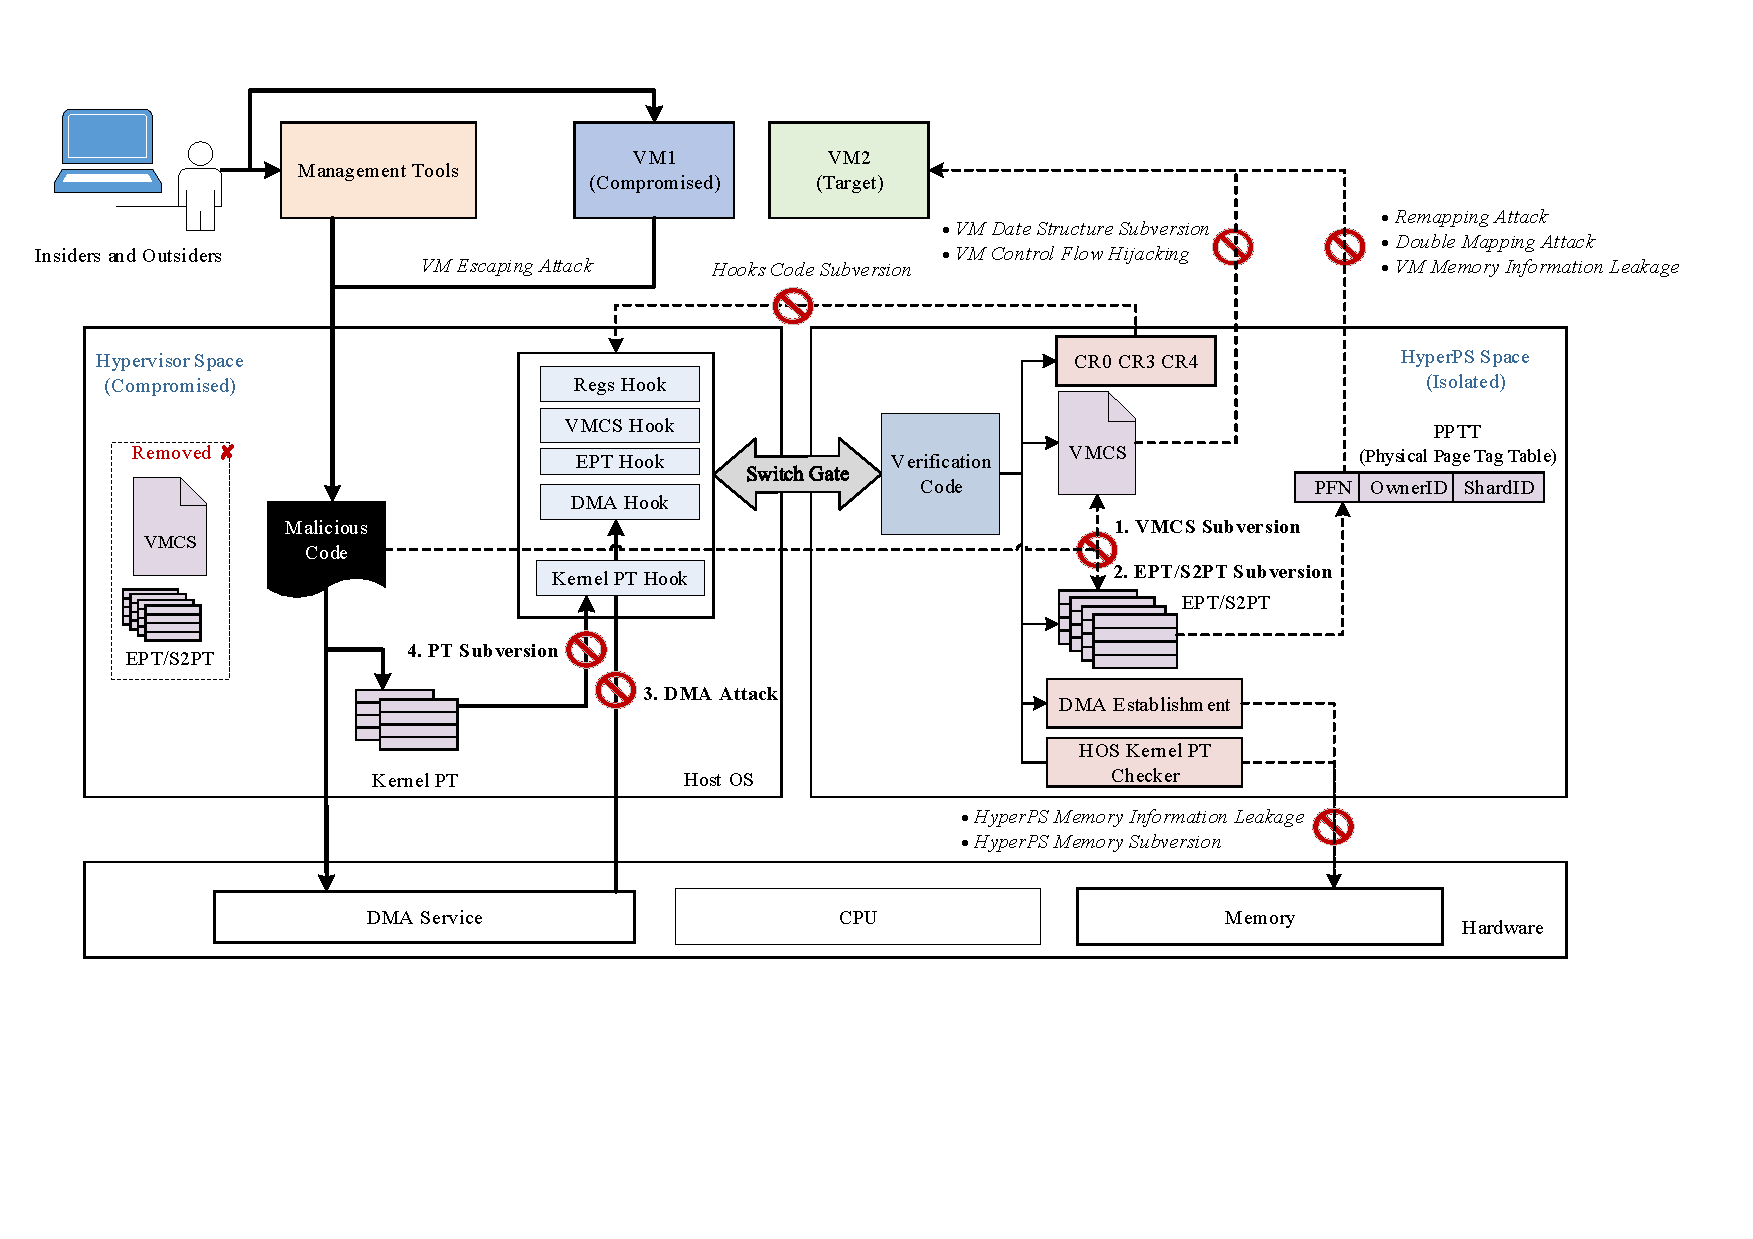
\includegraphics[width=1\textwidth]{IMG/panorama.pdf}
    \caption{The Panorama View of HyperPS. \\ HyperPS is committed to protect guest virtual machine under the compromised HostOS/Hypervisor. Privileges to manage VMCS and EPT are stripped from the compromised HostOS/Hypervisor into a separated and secure execution environment: HyperPS Space. The HyperPS space shares the same processor privilege as the HostOS. HyperPS does not rely on any special hardware or a higher privilege. Updates to VMCS and EPT are abandoned by the HyperPS, if the operations are not authorized or are adjudged as harmful to virtual machine.}
    \label{pic:panorama}
\end{figure*}

\subsection{Motivation} \label{sub:motivation}

\iffalse
#######################
###### 写作分析 ####### 
#######################
我们为什么要提出这个观点?首先明白一点:我们是站在VM角度上来思考问题的吗?假如VM不信任下面的VMM,那么就不应该上云,任何安全都不能保证。那么VM租户的角度是否能要求下面提供一个更加安全的架构,应该,但是不应该是租户要求下面的云服务提供商来采用我们的架构,因为一旦是要上云了,人家提供了什么你就选择什么,不能要求其更改云的架构。所以,站的视角一定不是VM租户的角度。那么角度就应该是下面的VMM。就是云服务提供商。对于VMM,其有什么动力要更改他们现在的架构?而不是现在的架构,毕竟无论如何一个同层隔离也更改了现有的云架构了。所以这里不应该假定存在内部攻击者,内部工作人员本身就知道我们的架构的存在,完全可以卸载了就好了,不需要还进行什么防护。所以,只可能存在一种情况,就是云服务提供商也不能完全保证其hostos的安全,但是其最核心的功能应该是如何保证其云的功能是安全的。所以,采用同层隔离的功能将云的相关功能隔离起来。从而实现云部分的安全。换句话说,就是,即使在HostOS存在脆弱点,其已经被攻击者攻陷的前提下,或者上面的VM通过虚拟机逃逸已经获取了下面的os的部分权限的前提下,如何保证VM的安全,即仍然能提供正常的云服务,保证用户的安全。那么前提就是云服务提供商也不完全信任下面的hostOS内核。
这段内容是否是我们的motivation?是,要详细写出来,但是思路不应该说VM租户内容,而应该从后面的内容出发,这个内容要不要在instruction中写出?要,但是要简洁,这里是详细说明。

基于上面的分析,我们假定的威胁模型应该是攻击者可以利用内核的脆弱性,获取了部分hostOS的权限,这权限是什么?这个要详细说明。
首先是最常见的,任意内存读写权限?或者特定的内存的读写权限?能否嵌入shellcode?这些要详细的分析,但是这个部分的工作放到后面,先将motivation写出来。

因为下面的Linux其实有很多脆弱点的,但是在传统的qemu-kvm的框架中,任何
这里首先要讲出如果HostOS并不安全,
The motivation for this work derives directly from
这部分要写出我们为什么要做这个系统,初衷是什么,要解决什么问题。

这部分要写什么?怎么写?
要按照这个逻辑来写:首先最开始用几句话说明云服务提供商最重要的任务是保证上面组会的安全,这是其需要负责的责任。然后需要论证hostos是不安全的,在这个条件下,其云系统可能被危害,一旦HOSTOS被危害,那么就无法保证上面VM的安全,立脚点一定是站在云服务提供商的角度上。最后自然而然的引出我们的motivation,就是如何在hostos被危害的前提条件下,云服务提供商如何保证虚拟机的安全。
\fi

\iffalse
##############################
##### Motivation中文初稿 #####
##############################
云服务商需要向云租户提供的众多服务中,能保证虚拟机的完整性和安全性是是其获取用户信任的关键因素。
对于每一台虚拟机,云服务提供商需要保证用户虚拟机的运行不会被侵害,其运算不会被恶意篡改,其数据不会被盗取。对于同属一个平台的不同服务器之间,云服务提供商需要保证不同虚拟机之间的有效隔离。但是,在QEMU-KVM架构中,作为HostOS的Linux不仅仅是一个负责提供虚拟化服务的hypervisor,还是一个正常的操作系统。
% HostOS在除了负责虚拟化相关核心功能之外,还是一个
即使云服务商采用定制的精简的Linux作为hostos,其仍然含有大量的与虚拟化功能无关的各种子系统subsystem,而这些功能,特别是来源复杂的内核驱动等不可避免的含有大量的可以被利用的内核脆弱点。这就提供给了攻击者一个巨大的攻击面surface,即使攻击者没有找到可以利用的QEMU/KVM脆弱点,其仍然可以通过exploit Linux其他subsystem的脆弱点实现对虚拟化部分的危害。云服务提供商并不能有效的保证Linux subsystem 特别是大量驱动设备的安全性,因此,云服务提供商需要进一步思考如何在hostos已经被危害的前提下保证虚拟机的安全,这就是HyperPS的motivation。
\fi

In this section, we discuss the motivations of why we need to protect VMs under an untrusted HostOS/Hypervisor.

Among the many services that cloud service providers need to provide to cloud tenants, ensuring the integrity and security of virtual machines is the key factor in gaining user trust. For each VM, the cloud service provider needs to ensure that the user's business in the VM will not be maliciously tampered with, and the data will not be stolen. For different VMs, cloud service providers need to ensure effective isolation between different VMs. However, in the QEMU-KVM architecture, Linux as HostOS is not only a hypervisor that is responsible for providing virtualization services, but also a normal operating system with full functions. In a real business deployment, even if cloud service providers adopt customized Linux as the HostOS, the Linux kernel still contains a large number of various subsystems that have nothing to do with virtualization. These subsystems, especially kernel drivers with complex sources, inevitably contain countless exploitable vulnerabilities. These subsystems provide the attacker with a huge attack surface. Even if the attacker does not find any exploitable QEMU or KVM vulnerabilities, he can still tamper with the virtualization component by exploiting the vulnerabilities of other Linux subsystems. Therefore, cloud service providers need a further think about how to ensure the security of VMs under the premise that the HostOS/Hypervisor has been compromised. This is the motivation of our HyperPS.


\subsection{Background}%
\label{sub:background}
This section presents some necessary background knowledge to facilitate readers to better understand HyperPS and threat model depicted in Figure \ref{pic:panorama}.
\subsubsection{QEMU-KVM}%
\label{ssub:qemu_kvm}
QEMU is a generic and open source machine emulator and virtualizer. QEMU can use other hypervisor like \verb|Xen| or KVM to use CPU extensions for virtualization. When used as a virtualizer, QEMU achieves near native performances by executing the guest code directly on the host CPU.
Kernel-based Virtual Machine (KVM) is an open source virtualization technology that converts Linux into a type-1 (bare-metal) hypervisor. KVM is a part of the Linux kernel that shares all the linux kernel's operating system-level components -such as the memory manager, process scheduler, security manager, and more to run VMs. Every VM is implemented as a regular Linux process, scheduled by the standard Linux scheduler, with dedicated virtual hardware like a network card, memory, and disks. KVM mainly consists of a loadable kernel module, kvm.ko, that provides the core virtualization infrastructure and a processor specific module, kvm-intel.ko or kvm-amd.ko.
In virtualization environment, KVM does not work on its own. It is only an API provided by the kernel for userspace. End users typically use KVM through QEMU where it is present as an acceleration method.
For the QEMU-KVM architecture, KVM interacts with QEMU (QEMU runs at the user space) in two ways: through device file \verb|/dev/kvm| and through memory mapped pages
% KVM interacts with user space - in most case QEMU - in two ways: through device file \verb|/dev/kvm| and through memory mapped pages.
Memory mapped pages are used for bulk transfer of data between QEMU and KVM. \verb|/dev/kvm| is the main API exposed by KVM. It supports a set of \verb|ioctl|s which allow QEMU to manage VMs and interact with them.
% 怎么引出HostOS的问题
% Since KVM is a part of the linux kernel, the Linux and the QEMU
% leverages the linux kernel's system-level



\subsubsection{VMCS}%
\label{ssub:vmcs}
Virtual-machine Control Structure is a data structure used in Virtual Machine eXtensions (VMX). It controls VMX non-root operations (guest virtual machine execution operations) and VMX transitions. Access to the VMCS is managed through the VMCS pointer (one per logical processor). The VMCS pointer is read and written suing the instructions \verb|VMPTRST| and \verb|VMPTRLD|. In general, the hypervisor configures a VMCS using \verb|VMREAD|, \verb|VMWRITE|, and \verb|VMCLEAR| instructions. A hypervisor could use a different VMCS for each virtual machine that it supports. For a virtual machine with multiple logical processor, the hypervisor could use a different for each logical processor. A logical processor may also maintain a number of VMCSs that are active, however, at any given time, at most one of the active VMCSs is the \textbf{current} VMCS. VMX instructions operate only on the \textbf{current} VMCS. 

%这段写的不好,没有写出危害的具体内容,应该突出VMCS就是唯一的接口,VM的所有的行为都是在VMCS的instruct下的
A compromised HostOS/hypervisor can force the guest virtual machine exit by tramper VM-Execution Control fields and VM-exit control fields in VMCS and tramper the guest virtual machine by writing Guest-State Area fields. 

% 一个被危害的hypervisor可以强迫虚拟机退出,并通过篡改其vmcs中的field等信息实现对guest VM 的危害。

% \subsection{Second Level Address Translation}%
% \label{sub:second_level_address_translation}
% Second Level Address Translation (SLAT) is a hardware-assisted virtualization technology which makes it possible to quick manage the physical memory without lots of VM exits. Extended Page Table (EPT) is the intel's implementation of SLAT, while ARM names its implementation as Stage-2 Page-tables.


\subsubsection{EPT}%
\label{ssub:ept}
Intel implements it Second Level Address Translation (SLAT) as Extended Page Table (EPT). 
EPT allows each virtual machine to manage its page table (not the EPT), without giving access to the underlying host machine's MMU Hardware. Thus, EPT reduces the need for hypervisor to keep syncing the shadow pages eliminating the overhead.
If EPT is enabled, guest-physical addresses are translated by traversing a set of EPT paging structures to produce physical addresses that are used to access memory.
In addition to translating a guest-physical address to a physical address, EPT specifies the privileges that software is allowed when accessing the address. Attempts at disallowed accesses are called EPT violations and cause VM exits.

A compromised HostOS/hypervisor could tramper EPT paging structures so that the virtual machine will execute arbitrary malicious code without knowing it. 
Moreover, a compromised HostOS/Hypervisor could access any data in the guest virtual machine with the help of virtual machine introspection.



%\subsection{Attacks and Threat Model} \label{sub:thretmodel}
\subsection{Attack Surface}\label{sub:attacksurface}
\iffalse
在这一章节中,我们首先给出攻击者的攻击路径,这个攻击路径并不需要单独画图,因为上面的图中已经阐释清楚了,攻击者有哪些方式可以危害虚拟机,只需要在图中更加明确的标识出来就可以了。然后再给出本文的威胁模型。

首先一句话尽可能简洁的描述出攻击者的攻击目的,

在这一章节中,我们首先描述在云环境中,攻击者如何攻击利用HostOS的漏洞实现对客户虚拟机的攻击。
其次,我们给出敌手的能力。
\fi

In this section, we first present how attackers tamper virtual machines through exploiting vulnerabilities in HostOS/Hypervisor. Then, we present several typical attack models/examples targeting at VMCS and EPT. At last, we explain some additional attacks (not attacks relative to virtualization components) depicted in Figure \ref{pic:panorama}.
%TODO 将图中的具体的攻击名称 1 2 3 4 等添加进去。
%At last, we illustrate the adversary's abilities. 

\subsubsection{How attacker subvert VM}
As illustrated in Section \ref{sub:background}, Hypervisor controls the execution of VMs through VMCSs, and manages VMs' physical memory through EPT. As such, these two data structures become the key target for adversary to tamper VMs. 
As depicted in Figure \ref{pic:panorama}, 
An adversary can exploit vulnerabilities to ``jail-break'' into the HostOS/Hypervisor, while he can subvert HostOS/Hypervisor by exploiting vulnerabilities in the HostOS kernel.
In this paper, we hypothesize the HostOS/Hypervisor has already been compromised, we attempt to protect VMs under the compromised HostOS/Hypervisor. 
After compromising the HostOS/Hypervisor, the attacker will inject malicious code to subvert VMs by tampering VMCSs and EPTs.
In details, we assume that the attacker can tamper VMCSs and EPTs with one of the following methods. First, the attacker can tamper any field in these two data structures with \verb|VMX| instructions, if the attacker has gained the root processor privilege. Second, the attacker can tamper these two data structures through direct memory write operations. The attacker can write these two data structures either through Direct Memory Access (DMA) or through regular memory access, if the attacker acquired these two data structures' memory locations before.  
%direct write to fields in these two data structures or 
%TODO 在这里要修改图,图中要添加内核的其他部分的功能,去掉内部管理者,保留虚拟机逃逸部分,同时对这部分的内容做虚线处理。

%这里,我们给出几个攻击模型,举例说明攻击者是如何危害上面的虚拟机的。

\subsubsection{Attack Examples}
We present several attacks to illustrate how an attack subvert VMs by through tampering VMCS and EPT.

\paragraph{VMCS Subversion}
Attackers can tamper fields of VMCS in VM Exit stage. For example, modifying the value of \verb|HOST_RIP| register and writing a malicious program address to this register will cause a control flow hijacking attack. Modifying the value of privilege register, CR0, will close the DEP mechanism, and modifying the value of CR4 register will close the SMEP mechanism.


\paragraph{EPT Subversion}
Malicious modification of EPT will break the isolation between virtual machines. A vicious VM can break the isolation between VMs by tampering with EPT entries, and access the memory of the victim VM at his vicious will. For example, the attacker can conduct remapping attack and double mapping attack to inspect a victim VM. 

For the double mapping attack, the attacker first controls and compromises a VM, then obtains the privilege of the hypervisor through the virtual machine escape attack, and maliciously accesses the VMCS structure to obtain the value of \verb|EPTP|. The attack process is as shown in Figure \ref{pic:remap}. 

In this way, the EPT address of the attacker virtual machine, VM1, and the victim virtual machine, VM2, are respectively obtained. And for a guest virtual address in VM2, A, the corresponding real physical address is B. For VM1, the real physical address corresponding to the guest virtual address C is D, then D is modified to be B by modifying the value of the last page item of EPT. Then VM1 can access the data of VM2 successfully, this process is called address double mapping.

For the remapping attack, there are VM1 (attacker) and VM2 (victim). A physical page (A) used by VM2 is released after being used. After A is released, VM1 remaps to A. So that the guest virtual address of VM1 points to the physical page A. By this way, VM1 can access the information on A used by VM2, causing information leakage.


\begin{figure}
    \centering
    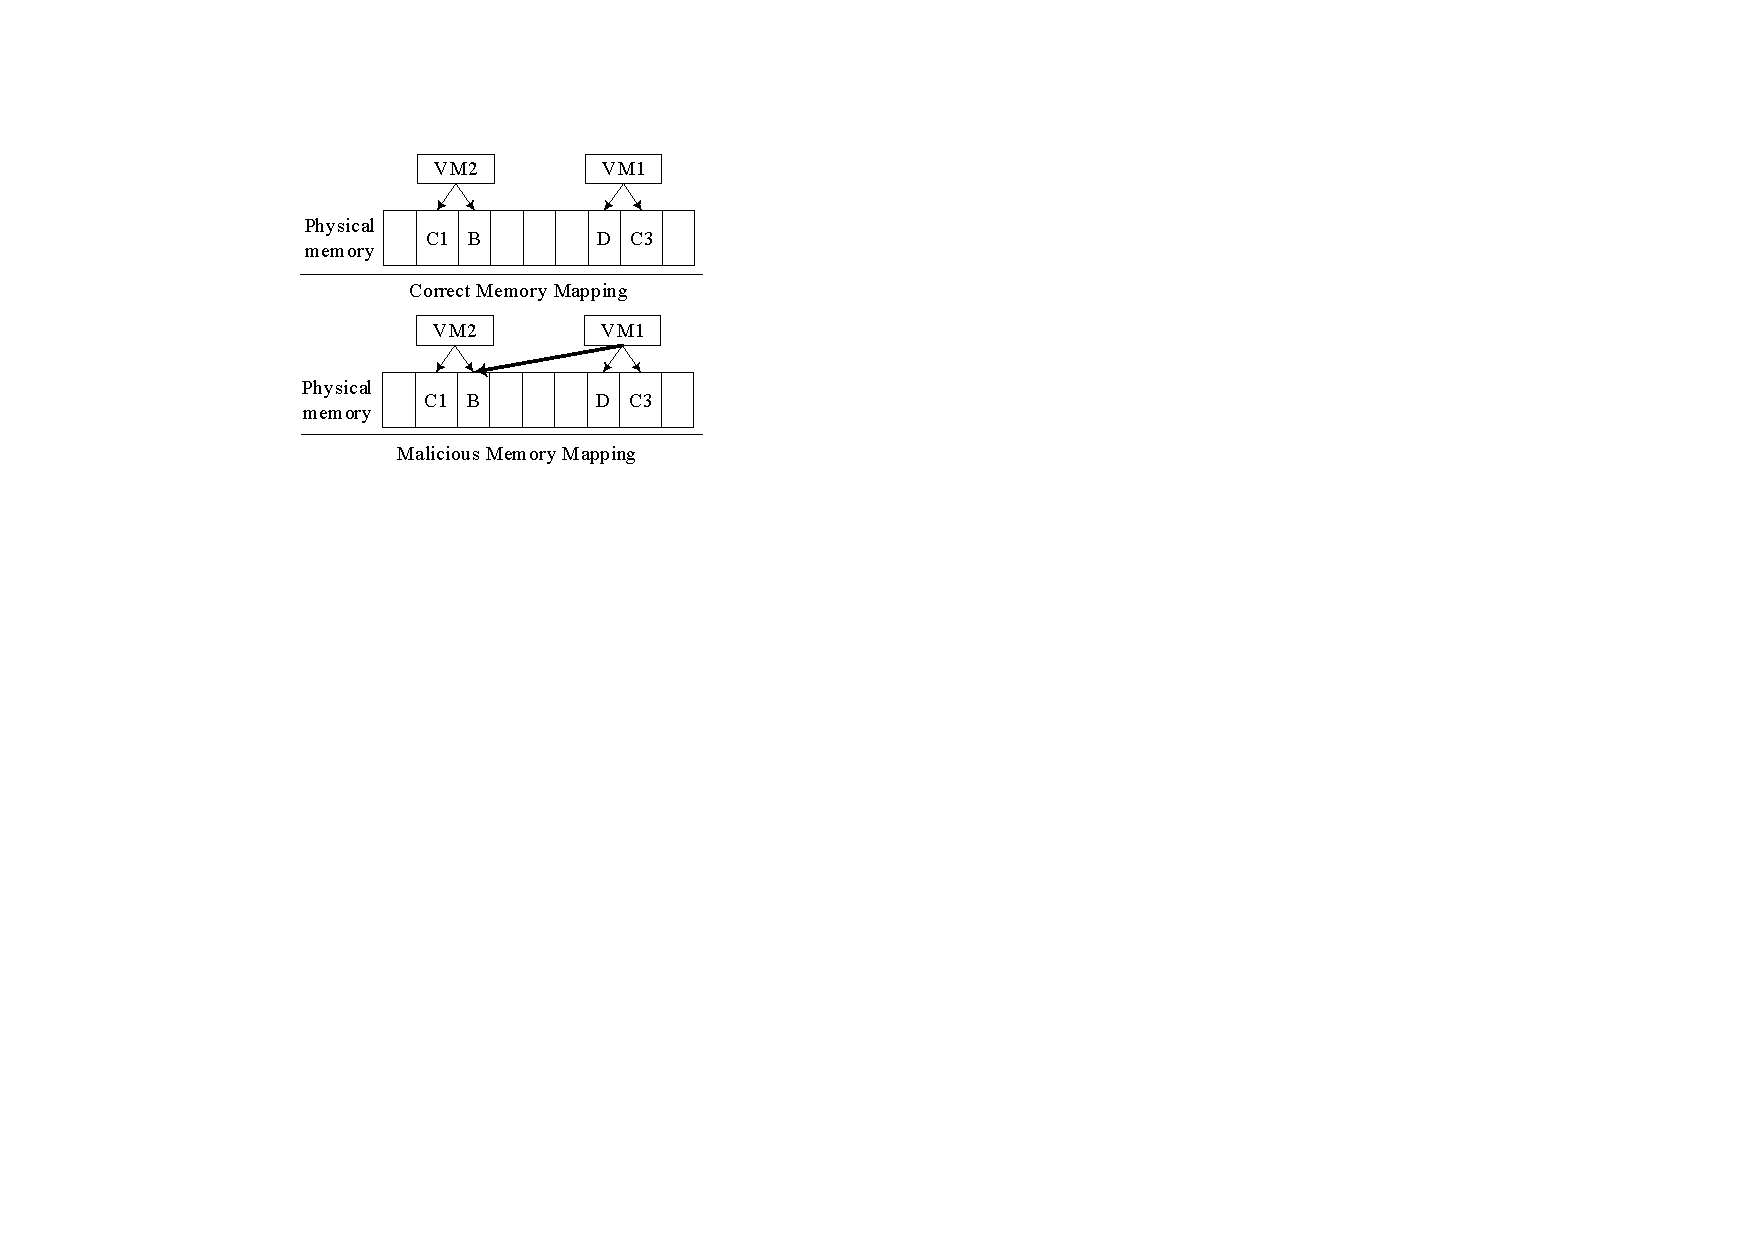
\includegraphics{IMG/remap.pdf}
    \caption{Diagram of Remapping Attack}
    \label{pic:remap}
\end{figure}

\subsubsection{Attacks to Kernel Page Tables}
We also take into account the fact that attacker already knows the deployment of HyperPS. As depicted in Figure \ref{pic:panorama}, key components, such as Kernel Page Tables, Control Registers, to create the secure and isolated execution environment are also protected by us. More details about the creation of the secure and isolated execution environment are illustrated in Section. 
%TODO 添加关于章节的引用
 
\subsection{Threat Model} \label{sub:threatmodel}
In this paper, 
We assume that the HostOS/Hypervisor has been compromised and controlled by the powerful adversary. The adversary can turn off kernel security mechanisms, such as DEP, SMEP, SMAP, and so on. The adversary can tamper fields of VMCSs and EPTs with dedicated malicious values. The adversary can also tamper VMCSs and EPTs through DMA write or regular memory access to them.  

We assume that the adversary does not possess the capability to conduct side channel attack and Hardware-based attack. We also assume that the adversary is unwilling to conduct the Denial of Service attack (DOS). In this paper, we assume that hardware resources are trusted, including processor, buses, BIOS/UEFI, and so on. 

%原威胁模型写的有问题。给出的两个例子后面写危害VMCS和

















\section{Design}%
\label{sec:desgin}

\iffalse
这一张将写本系统是如何设计的,主要内容分为两部分:一部分是如何hook。另外一部分是如何实现对各种数据结构的保护。

本文的特权特指就是内存管理,管理VMCS的原因就是里边含有EPTP,其余的域并不进行保护。

那么文章的核心就是剥夺了VMM管理物理内存的权限,这就是HyperPS的P的内容。
那么针对这一特点,这一思路,设计要怎么写。
要说明如下的几个问题:1. 如何分离权限,即VMM管理内存都是靠什么实现的,特权的实现途径是啥,怎么将这些特权分离。这里要写出两个东西:1.1 原本的VMM对内存管理的相关函数被Hook,所有的操作都无法在VMM中实施,即完成了HOOK。1.2 为了防止攻击者直接修改EPT paging structure,这就是将EPT从常规的空间中移除。
这两个点要顺序换过来,先写移除,再写hook。
2. 第二要写怎么实现保护,在hook完成后,剥离了VMM对物理内存的管理,HyperPS是如何实现对内存的管理的。这里要假如关于缺页中断的相关内容,怎么处理EPT异常,也要处理新建EPT的内容,也要包括不同虚拟机的映射关系,也要绑定EPT与VM的关系,不允许VM和VMM更改EPTP内容。

上面的1 2就是两段的内容,首先要给出一个overview,讲整个框架的结构。

##################
开头内容中文初稿
##################
这一节,我们首先提出我们的HyperPS,我们详细描述HyperPS的构成组件。然后我们详细阐述了HyperPS是如何剥离原VMM对内存的管理权限的。最后我们提出HyperPS是如何实现对内存的保护,从而实现保护虚拟机的运行以抵御一个受危害的VMM。
讲HyperPS如何实现对物理内存的管理。
\fi
In this section, we first propose the architecture of HyperPS. Then, in the following subsection, we elaborate on how HyperPS stripped the compromised HostOS kernel's privilege of managing guest VM's memory and the physical memory. Finally, we illustrate how HyperPS manages the guest VM's memory and physical memory to resist the compromised HostOS/Hypervisor.


\subsection{HyperPS Overview}%
\label{sub:hyperps_overview}

% 首先一句话说明HyperPS要做什么,然后Figure depict the details on the architecture of HyperPS.
% As shown in Figure, 我们创造了一个同层隔离空间用于履行原本属于compromised HostOS的管理虚拟机物理内存的权力。


% We present HyperPS to protect guest virtual machines against compromised Hypervisor. In virtualization environment, the hyperivor deprivileges the guest VM’s kernel and interposes all interactions between guest VMs and the physical memory. Neither isolation between VMs nor virtual-physical mapping relationships in a VM will inevitable be tamperred if the Hypervisor has been compromised. HyperPS, thus, deprives the Hypervisor of privileges on managing physical memory.

In a virtualization environment, the HostOS/Hypervisor deprivileges the guest VM’s kernel and interposes all interactions between guest VMs and the physical memory. 
If the HostOS/Hypervisor has been compromised, both isolation between VMs and virtual-physical mapping relationships for a VM will inevitablely be tampered. 
Thus, in this paper, we present HyperPS to deprive the Hypervisor of privileges on managing physical memory.

% Neither isolation between VMs nor virtual-physical mapping relationships in a VM will inevitable be tamperred if the Hypervisor has been compromised.

Figure \ref{fig:design} depicts the details on the architecture of HyperPS. 
Firstly, the compromised HostOS/Hypervisor is stripped of privileges of managing physical memory. 
As shown in Figure \ref{fig:design}, original functions about physical memory management (e.g., EPT operations, EPTP switching operations, and some VMCS operations) in the compromised Hypervisor are hooked into the HyperPS Space. 
% However, it is far from sufficient to just hook these functions
However, hooking these functions is far from sufficient to deprive the HostOS/Hypervisor of the capabilities of managing physical memory completely.
% Firstly, as shown in Figure \ref{fig:design}, HyperPS deprives the compromised HostOS kernel/Hypervisor with privileges of managing physical memory.
% Firstly, as shown in Figure \ref{fig:design}, we create a delicate kernel-level secure and isolated execution space, called HyperPS Space, to inherit privileges of managing physical memory that originally belonged to the compromised Hypervisor.
% Original functions about physical memory management (e.g., EPT operations, EPTP switching operations, and some VMCS operations) in the compromised Hypervisor are hooked into the HyperPS Space.
% There are still some extraordinary cases that attackers can subvert memory management data structures by using regular memory access. For example, attackers can inject newly malicious VMX assembly code so that all hooked functions will be bypassed.
There are still some extraordinary cases in which attackers can subvert memory management data structures. For example, attackers can inject newly malicious VMX assembly code so that all hooked functions will be bypassed. The attacker can also access memory management data structures by using regular memory access if he gets their locations in advance.
% can bypass the hooked functions by introducing new malicious VMX assembly code.
HyperPS, in consideration of these cases, removed VMCS and EPT from the original Hypervisor space and placed them in the HyperPS Space. 
% For cases where attackers subvert memory management data structures by using regular memory access, and cases where attackers bypass the hooked functions by introducing new malicious VMX assembly code
% use regular memory access to tamper with
% For cases where an attacker uses regular memory access or newly introduced malicious VMX assembly code to bypass the hooked functions and tamper with the relevant memory management data structures, HyperPS removed VMCS and EPT, which are crucial to virtualization, from the original Hypervisor space and places them in the HyperPS Space.
Secondly, in the HyperPS Space, we introduce two new data structures, called Page-Mark structure and VM-Mark structure, to tag the mapping relations between the physical frames and the virtual machines. With the help of these two data structures, even if an attacker can tamper EPT Paging-structures with malicious value through a legal function invocation, HyperPS can still effectively detect such attacks and resist them.
Lastly,as shown in Figure \ref{fig:design}, we create a delicate kernel-level secure and isolated execution space, called HyperPS Space, to inherit privileges of managing physical memory that originally belonged to the compromised Hypervisor. We adopt a set of techniques to guarantee the isolation of the HyperPS Space. Context switching from the compromised HostOS kernel/Hypervisor to the HyperPS Space exclusively passes through a designated Switch Gate. Actually, the Switch Gate is the only interface between the Normal Space and the HyperPS Space.

%图中的内容添加虚拟机退出的线,removed的字段加粗 pptt是表 修改成表的形式

\begin{figure*}[htpb]
    \centering
    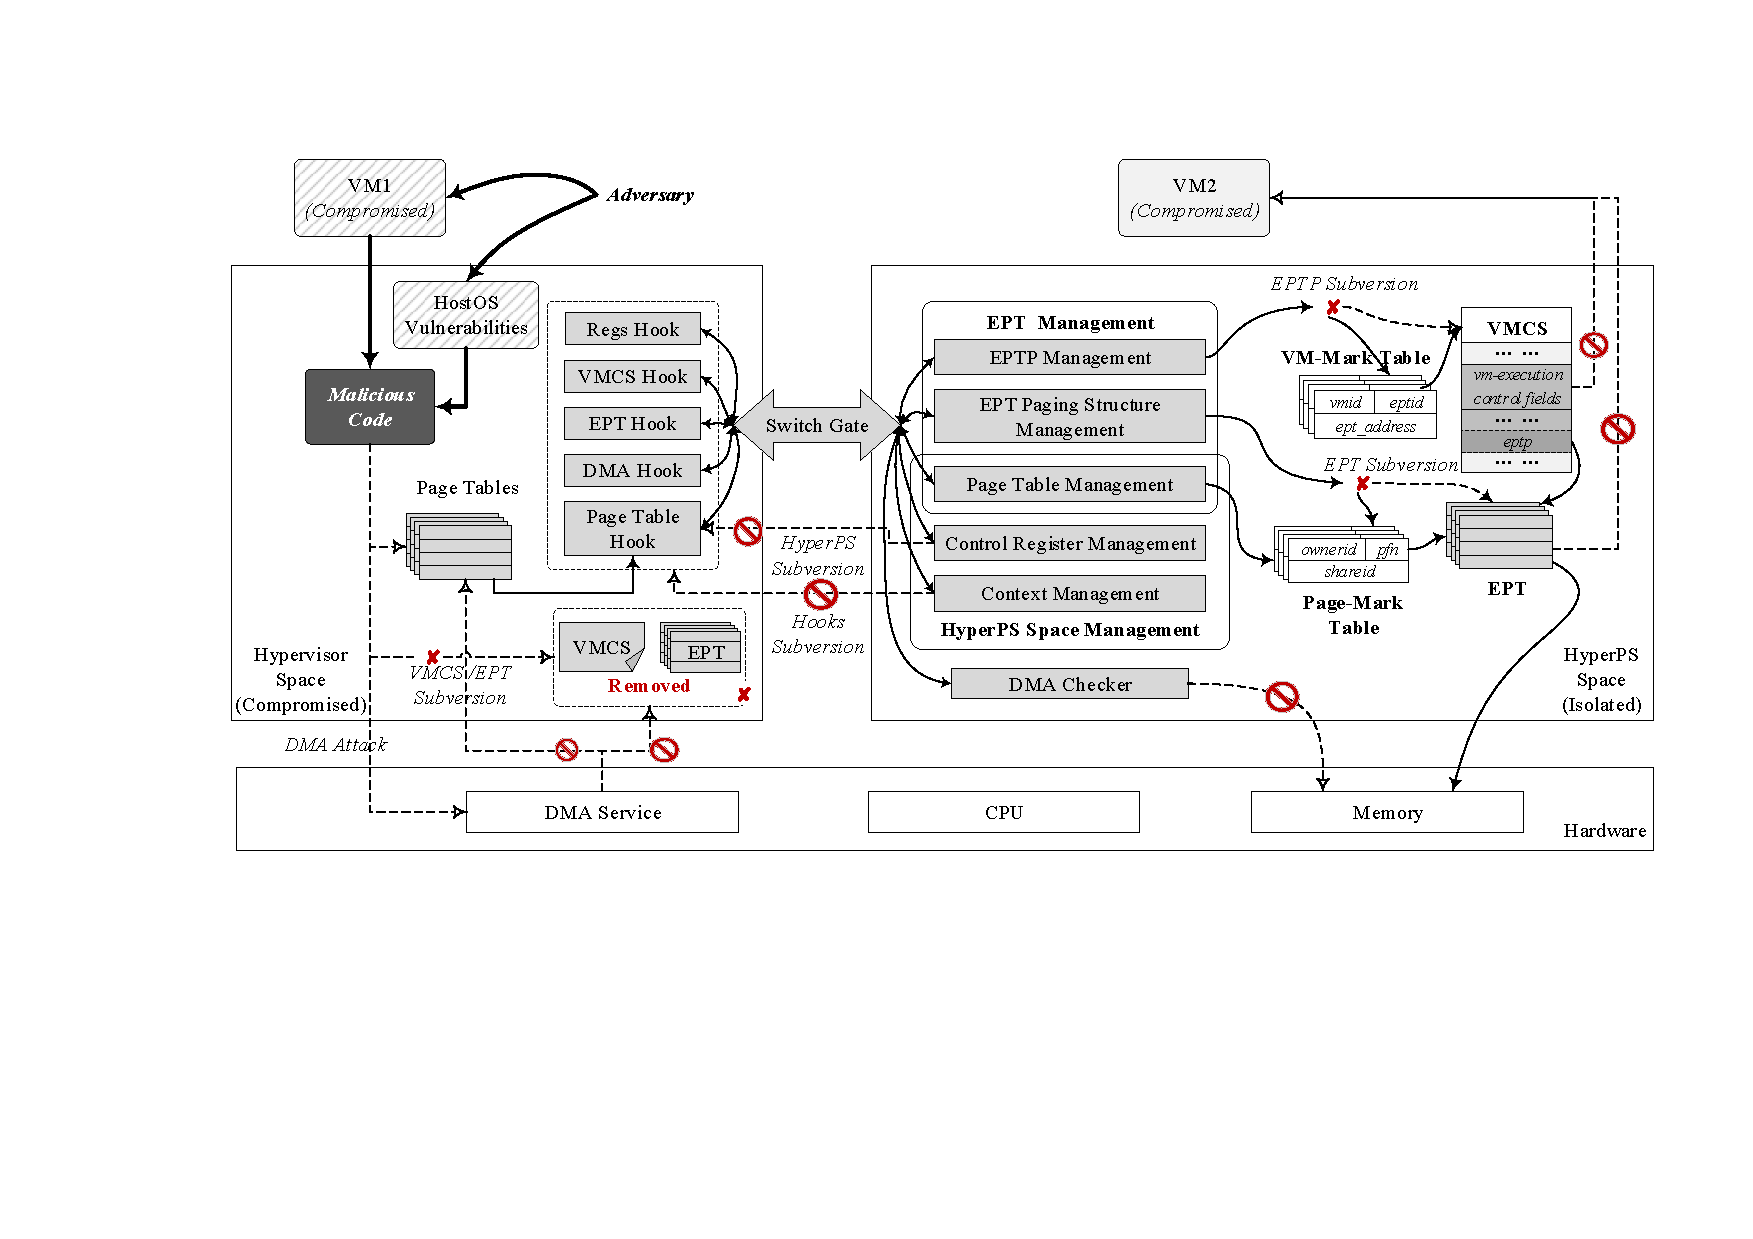
\includegraphics[width=0.9\linewidth]{IMG/newdesign.pdf}
    \caption{HyperPS Architecture  \\ HyperPS is committed to protect guest virtual machine under the compromised HostOS/Hypervisor. Privileges to manage VMCS and EPT are stripped from the compromised HostOS/Hypervisor into a separated and secure execution environment: HyperPS Space. The HyperPS Space shares the same processor privilege as the HostOS. HyperPS does not rely on any special hardware or a higher privilege. Updates to VMCS and EPT are abandoned by the HyperPS, if the operations are not authorized or are adjudged as harmful to virtual machine.}%
    \label{fig:design}
\end{figure*}



\iffalse
那么文章的核心就是剥夺了VMM管理物理内存的权限,这就是HyperPS的P的内容。
那么针对这一特点,这一思路,设计要怎么写。
要说明如下的几个问题:1. 如何分离权限,即VMM管理内存都是靠什么实现的,特权的实现途径是啥,怎么将这些特权分离。这里要写出两个东西:1.1 原本的VMM对内存管理的相关函数被Hook,所有的操作都无法在VMM中实施,即完成了HOOK。1.2 为了防止攻击者直接修改EPT paging structure,这就是将EPT从常规的空间中移除。
这两个点要顺序换过来,先写移除,再写hook。
2. 第二要写怎么实现保护,在hook完成后,剥离了VMM对物理内存的管理,HyperPS是如何实现对内存的管理的。这里要假如关于缺页中断的相关内容,怎么处理EPT异常,也要处理新建EPT的内容,也要包括不同虚拟机的映射关系,也要绑定EPT与VM的关系,不允许VM和VMM更改EPTP内容。
\fi

\subsection{Privilege Separation}%
\label{sub:privilege_separation}

\iffalse
首先要讲管理内存的权限是通过EPT实现的,要实现特权的分离,分为两步,一是将EPT从原有空间移除,使得原有的Hypervisor无法直接access数据结构。第二步是对能access这些数据结构的函数进行验证。
% 将移除操作这些数据结构的逻辑。
在传统的没有HyperPS的虚拟化环境中,Hypervisor 通过EPT直接管理管理内存
这里要先讲为什么要将EPT和VMCS从原有的空间移除,然后再讲怎么移除。移除以后存在疑问,就是会造成PANIC, 如何解决,就是hook的问题,
The EPT mechanism is a feature that can be used to support the virtualization of physical memory. 
EPT defines a layer of address translation that augments the translation of linear addresses. 
When EPT is in use, certain addresses that would normally be treated as physical addresses (and used to access memory) are instead treated as guest-physical addresses. Guest-physical addresses are translated by traversing a set of EPT paging structures to produce physical addresses that are used to access physical memory.
It's EPT mechanism that treat guest-physical address like a virtual address and the EPTP is the CR3.
We should write (\verb|VMWRITE|) EPTP to the VMCS. 
\fi

% According to the Intel manual, the EPT mechanism is a core feature that is used to support the virtualization of physical memory.
EPT defines a layer of address translation that augments the translation of linear addresses. 
When EPT is in use, the EPT interposes all memory access between guest VMs and the physical memory. 
Certain addresses that would normally be treated as physical addresses (and used to access memory) are instead treated as guest-physical addresses. Guest-physical addresses are translated by traversing a set of EPT paging structures to produce physical addresses that are used to access memory.
% If the hyperivor has been subverted by the attacker,
If attackers have gained control over a Hypervisor, 
neither isolation between VMs nor virtual-physical mapping relationships in a VM are immune to them. 
% Attackers can modify any EPT paging structures with any values.
In this paper, HyperPS deprives the Hypervisor's privileges of managing physical memory by limiting it from accessing and managing all EPTs. 
Figure \ref{fig:inter} depicts the difference in the VM-Exit handling between the traditional system and the system with HyperPS.
\begin{figure}[htpb]
    \centering
    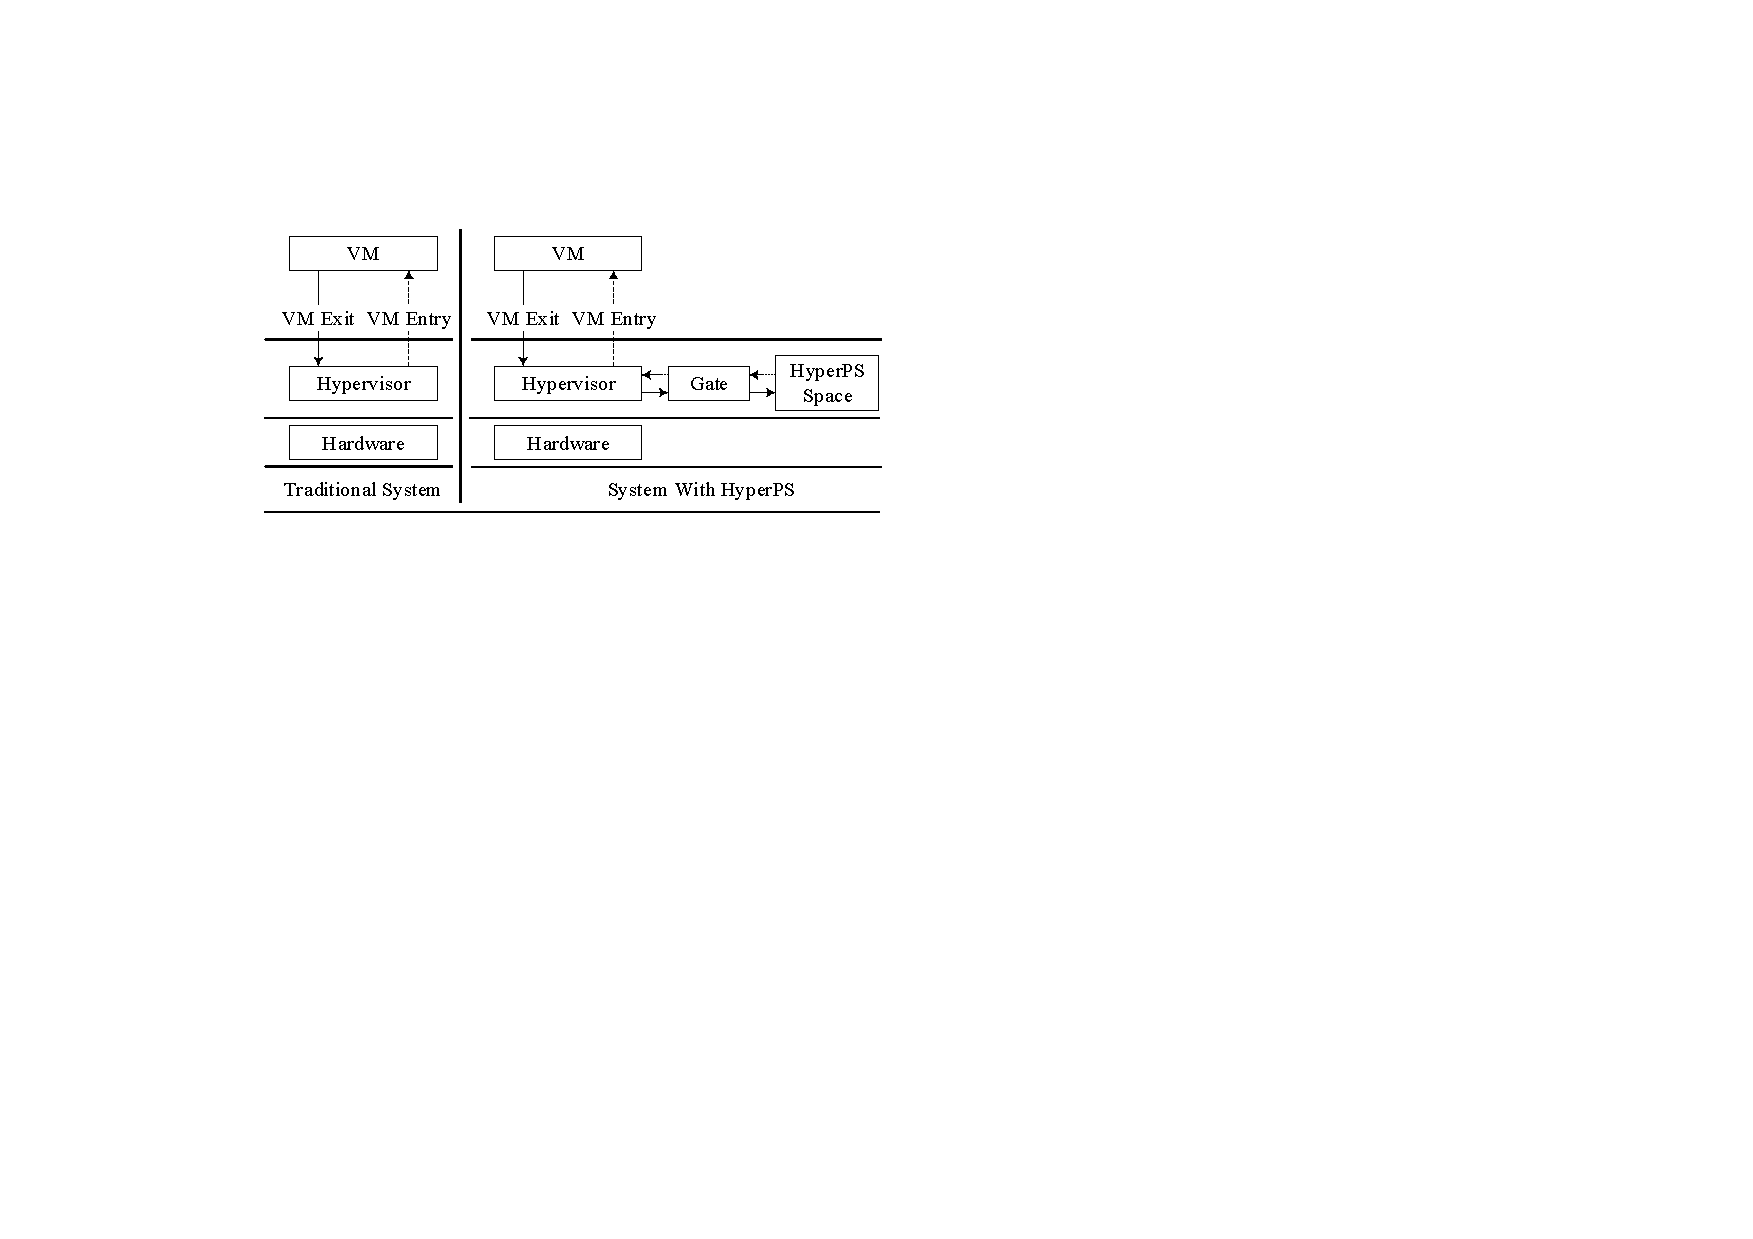
\includegraphics[width=0.8\linewidth]{IMG/interaction.pdf}
    \caption{Interaction Difference between the traditional system and system with HyperPS \\ VM-Exit handling only involves the Hypervisor in traditional system. In the system with HyperPS, VM-Exit is redirect into the HyperPS Space through the Gate. Context Management during VM-Exit and VM-Entry is managed by the HyperPS.}%
    \label{fig:inter}
\end{figure}


% Exception handle
% all code and any data in guest
% any VM's content in memory can no longer be
% EPT paging structures
% neither isolation between VMs nor virtual-physical mapping relationships in a VM
% nor
% In this paper, HyperPS deprives the compromised hyperivor with privileges of managing physical memory by limiting it from accessing and managing all EPTs.
% deprives the virtual machine
% 上面的内容说明了要限制权限是通过EPT来实现的。怎么移除EPT 为什么要移除VMCS
\iffalse
首先要讲管理内存的权限是通过EPT实现的,要实现特权的分离,分为两步,一是将EPT从原有空间移除,使得原有的Hypervisor无法直接access数据结构。第二步是对能access这些数据结构的函数进行验证。
% 将移除操作这些数据结构的逻辑。
在传统的没有HyperPS的虚拟化环境中,Hypervisor 通过EPT直接管理管理内存
这里要先讲为什么要将EPT和VMCS从原有的空间移除,然后再讲怎么移除。移除以后存在疑问,就是会造成PANIC, 如何解决,就是hook的问题,
It's EPT mechanism that treat guest-physical address like a virtual address and the EPTP is the CR3.
we should write (VMWRITE) EPTP to the VMCS. 
\fi


Firstly, HyperPS removed all EPTs and VMCSes from the Hypervisor space. EPT manages all physical memory of the VM, as mentioned above, HyperPS removed them from the Hypervisor space. However, there is a hardware register, called Extended Page Table Pointer (EPTP), that contains the address of the base of EPT table, as well as EPT configuration information. Simple obliteration of EPT would make EPTP error which will crash the whole virtualization environment too. 
Besides, the VMCS records the value of EPTP in the VM-Execution Control Fields. The processor will load the value in that field into the hardware register when VM-Entry. 
Even if the attacker cannot directly tamper with EPTs, he can also subvert the guest VMs by tampering with a malicious EPTP value in the VMCS. Thus, HyperPS removed all VMCSes from the Hypervisor too. 
% The adversary can tamper with the EPTP value in the VMCS to make the VM use a new set of malicious EPT table.
% Thus, HyperPS
% A Hypervisor load the value
% EPTP is a hardware register that works like the CR3 register in traditional memory translation. It always points to the
% The VMCS stores the value of EPTP in the VM-Execution Control Fields.
% VMCS store EPTP that points to EPT
% EPTP works like the CR3 in

Secondly,  HyperPS hooks all VMCS operation and EPT operation functions in the Hypervisor into the HyperPS Space.
In the QEMU-KVM architecture, The KVM provides a wrapper around privileged instructions and is responsible for executing privileged instructions.
The QEMU does not need to deal architecture specific details, it just needs to invoke KVM functions with proper parameters. 
HyperPS hooks KVM's VMCS and EPT functions into the HyperPS Space. In the HyperPS Space, Context Management in the HyperPS Space Management component checks the invoked parameters and verifies if the inputted parameters are legal or not.  
% Based on Intel manuals, VMCS can only be manipulated by privileged instructions: \verb|VMCLEAR| \verb|VMPTRLD|, \verb|VMREAD|, \verb|VMWRITE|, and so on.
% In the QEMU-KVM architecture, the KVM is responsible for executing these privileged instructions. The KVM provdes a wrapper around these privileged instructions. The QEMU does not need to deal architecture specific details, it just need to invoke KVM functions with proper parameters.
% For example, \verb|vmcs_writel()| wraps the privileged instruction \verb|VMWRITE|, and \verb|vmcs_readl()| wraps the privileged instruction \verb|VMREAD|.
% HyperPS hooks these functions into the HyperPS Space. In the HyperPS Space, Context Management in the HyperPS Space Management component check the invoked parameters and verifies if the write to \verb|VM-Execution Control Fields.EPTP| is legal or not.
Since VMCS is hidden in the HyperPS Space which is accessible by functions in the Hypervisor space, all context management (accessing VMCS operations) will be trapped int HyperPS Space inevitably.
% inevitablely.
%During VM-Exit (codes to access VMCS can only be executed in VM-Exit), the Hypervisor 
EPT operation functions are also hooked into the HyperPS Space too. EPT operation functions are different from VMCS operation functions, for the VMCS can only be accessed by just a few privileged instructions. Instead of hooking EPT accessing functions, HyperPS hooks all EPT operation functions. Functions about EPT creation, load, traversal, update and destruction are re-placed into the HyperPS Space. Functions that invoke these EPT operation functions are hooked into the HyperPS Space.

% operation functions
% HyperPS checks the
% provide a wrapper around these privileged instructions.
% are responsible
% HyperPS hooks functions that contain these instructions.
% In specific,
% at each time when VM exits to the Hypervisor, HyperPS
% VMCS operation and EPT operation functions certainly involve privileged instructions.
% On a privileged instruction, it switches back to the KVM kernel module,

Lastly, HyperPS also takes DMA attacks into consideration. An attacker with the ability of arbitrary memory access by exploiting DMA vulnerabilities can tamper VMCSes and EPTs. IOMMU carries out access control for DMA access. Thus, in this paper, HyperPS employs IOMMU mechanism to resist DMA attacks.
In the Hypervisor space, HyperPS found out all the critical data used by IOMMU, and removed the corresponding page table entries that map these data from the page tables. In this paper, HyperPS mainly defines the entrance address of HyperPS, the Page-Mark data, and the VM-Mark data (details about Page-Mark and VM-Mark data structure are illustrated in Section \ref{ssub:eptp_protection}) as the critical data.
In the HyperPS Space, HyperPS intercepts the address mapping function about I/O. At runtime, HyperPS verifies whether the address belongs to the HyperPS Space on receiving signals of executing these IO functions. 


% HyperPS removed all corresponding page table entries that map
% mapping of the critical data from the page table which IOMMU uses.
% In the HyperPS Space, DMA Management Component
% In this paper, HyperPS employs IOMMU mechanism to resist DMA attacks. IOMMU carries out access control for DMA access.

% \subsection{VM Memory Protection}%
% \label{sub:vm_memory_protection}
\subsection{Privilege Management}%
\label{sub:privilege_management}



\iffalse
那么文章的核心就是剥夺了VMM管理物理内存的权限,这就是HyperPS的P的内容。
那么针对这一特点,这一思路,设计要怎么写。
要说明如下的几个问题:1. 如何分离权限,即VMM管理内存都是靠什么实现的,特权的实现途径是啥,怎么将这些特权分离。这里要写出两个东西:1.1 原本的VMM对内存管理的相关函数被Hook,所有的操作都无法在VMM中实施,即完成了HOOK。1.2 为了防止攻击者直接修改EPT paging structure,这就是将EPT从常规的空间中移除。
这两个点要顺序换过来,先写移除,再写hook。
2. 第二要写怎么实现保护,在hook完成后,剥离了VMM对物理内存的管理,HyperPS是如何实现对内存的管理的。这里要假如关于缺页中断的相关内容,怎么处理EPT异常,也要处理新建EPT的内容,也要包括不同虚拟机的映射关系,也要绑定EPT与VM的关系,不允许VM和VMM更改EPTP内容。
\fi

HyperPS has removed EPTs and VMCSes from the original Hypervisor space, and functions about accessing and updating them have also been hooked into the HyperPS Space. 
The HostOS/Hypervisor has already been deprived of privileges of managing the physical memory directly. Actually, the HostOS/Hypervisor can not access EPTs and VMCSes with regular memory access instructions or DMA instructions. 
However, the HostOS/Hypervisor could still retrieve details about EPTs and VMCSes through legal functions. 
The attacker can also tamper with EPT Paging-structures and VMCS fields with malicious input to these hooked functions.
In this paper, HyperPS present two tables : Page-Mark Table and VM-Mark Table, to tag the mapping relations between the physical memory page frames and the virtual machines. Page-Mark Table consists of Page-Mark structure, while VM-Mark Table consists of VM-Mark structure.

\subsubsection{EPTP Protection}%
\label{ssub:eptp_protection}
In this paper, we propose a table: VM-Mark Table to restrict Hypervisor from loading an unverified EPTP value arbitrarily.
The VM-Mark Table consists of VM-Mark structures. 
In the Hypervisor, a new EPTP means a different EPT Paging-structure hierarchy. An attacker can map VM virtual address to a totally new physical page frame that holds malicious code. In this paper, HyperPS hooks all functions that can switch the value of EPTP and verifies if the value is authorized by HyperPS before. HyperPS relies on the VM-Mark structure to identify whether the operation of changing EPTP is legal or not. 

Table \ref{tb:vmmark} presents the basic architecture of the VM-Mark structure.
The field \verb|VMID| is a magic number randomly generated when the VM is created. 
The field \verb|EPTID| is also a magic number randomly generated when the EPTP is allocated.
In a virtualization environment,
the Hypervisor can use a different VMCS for each virtual machine that it supports. However, these VMCSes share the same EPTP value for a single VM. 
HyperPS, thus, blinds the different EPT with a VM identifier instead of each VMCS.
HyperPS also takes \verb|VMFUNC| into consideration too. EPTP switching is VM function 0. This VM function allows VM in VMX non-root operation to load a new value for the EPTP. The EPTP switching operation does not incur VM-Exit to VMX root operation.
The \verb|VMFUNC| is limited to selecting from a list of potential EPTP values configured in advance by the Hypervisor in VMX root operation. Thus, HyperPS also hooks all functions that manage the EPTP list in VMX root operation.

When the Hypervisor is going to load a new value for the EPTP or change the EPTP list in VMX root operation, functions are hooked and control flow is redirected to HyperPS Space. 
HyperPS iterates the VM-Mark table to check if the EPTP is authorized in advance.

% checks if the input EPTP value matches a entry in
% EPTP in VMX root operation or change
% In this paper, HyperPS
% EPTP switching is VM function0. This VM function allows software in VMX non-root operation to load a new value for the EPT pointer (EPTP), thereby establishing a different EPT paging-structure hierarchy. Software is limited to selecting from a list of potential EPTP values configured in advance by software in VMX root operation.
% When switching from one VM to another, the Hypervisor writes the same EPTP value into all the VMCSes for a single VM.
% These VMCSes share the same EPT
% Different VMCS that
% HyperPS blinds the EPT with the VM identifier instead of the VMCS.
% HyperPS blinds EPTs with VM identifiers

\begin{table}[]
    \caption{VM-Mark Structure}
    \resizebox{\linewidth}{!}{
\begin{tabular}{l|l|l|l}
\hline
\textbf{Label}       & \multicolumn{1}{c|}{VMID} & \multicolumn{1}{c|}{EPTID} & \multicolumn{1}{c}{EPT\_Address} \\ \hline
\textbf{Description} & The VM Identifier         & The EPT Identifier         & The Entry Address of this EPT    \\ \hline
\end{tabular}}
    \label{tb:vmmark}
\end{table}

% unauthorized EPTP
% EPTP switching is VM function0. this VM function allows software in VMX non-root operation to load a new value for the EPT pointer (EPTP), thereby establishing a different EPT paging-structure hierarchy. Software is limited to selecting from a list of potential EPTP values configured in advance by software in VMX root operation.
% VM-mark的作用是保证VM 和对应的EPT 是对应的,攻击者无法通过更换新的EPT表实现对虚拟机的攻击。
% Page-mark的作用是用于虚拟机内部的隔离。

\subsubsection{EPT Paging-structure Protection}%
\label{ssub:ept_paging_structure_protection}
Values that update to EPT Paging-structures need to be verified too. In this paper, we present Page-Mark structure to record the relationships between EPT Paging-structures and the physical memory page frames. In HyperPS Space, HyperPS composes all Page-Mark structures into one table, called Page-Mark Table.
HyperPS guarantees effective isolation between different virtual machines based on this Page-Mark Table. 

Table \ref{tb:pagemark} presents the basic architecture of the Page-Mark structure.
The field \verb|PFN| is the first address of the physical memory page frame. HyperPS fills in this field when a physical memory page frame is assigned to a VM. Usually, the Hypervisor will create a new EPT Paging-structure that maps this page frame and assigns the physical memory page frame to a guest physical memory page frame. The field \verb|OwnerID| is the same as the value of \verb|VMID| that identifies different VM/EPT. At the time when a physical memory page frame is assigned to a VM, HyperPS fills the field \verb|OwnerID| with the value of the corresponding \verb|VMID|. 
Kernel Same-page Merging (KSM), used by the KVM, allow for a greater guest density of identical or similar guest operating system by avoiding memory duplication.
% KVM guests to share identical memory pages
% However, In some virtualization environment, some particular physical memory page frames may be shared between differnt VMs.
For example, different VMs with the same kernel may share the same physical memory page frames that hold the kernel code. HyperPS takes this situation into consideration too. If one physical memory page frame is shared between VMs, HyperPS fills the field \verb|SharedID| with the one of the VM's \verb|OwnerID|. More details about \verb|Page-Mark Structure| are illustrated in Section \ref{sub:ksm_handle}.

HyperPS has hooked all functions about EPT operations.
At runtime, control flow will be redirected to the HyperPS Space when the Hypervisor invokes these functions. 
In the HyperPS, HyperPS index the Page-Mark structure tables with the physical memory page frame address. 
HyperPS ensures that any update to EPT Paging-structures must be in line with records in the Page-Mark Table.
With the help of the Page-Mark Table, the attacker can no longer map a physical memory page frame that initially belongs to a victim VM to the malicious VM. The compromised Hypervisor can not map the guest VM into a dedicated physical memory page frame anymore. 
% If the update to EPT
% HyperPS will verify the owner of pages when EPT update
% HyperPS has hooked all functions about EPT operations. On executing thses functions, control flow is redirect into the HyperPS Space.

\begin{table}[]
    \caption{Page-Mark Structure}
    \resizebox{\linewidth}{!}{
\begin{tabular}{l|l|l|l}
\hline
\textbf{Label}       & \multicolumn{1}{c|}{OwnerID} & \multicolumn{1}{c|}{SharedID} & \multicolumn{1}{c}{PFN}                                                                  \\ \hline
\textbf{Description} & The Owner Identifier         & The Shared Identifier         & \begin{tabular}[c]{@{}l@{}}The Address of the Physical \\ Memory Page Frame\end{tabular} \\ \hline
\end{tabular}}
    \label{tb:pagemark}
\end{table}

% the attribution of different physical memory page frames.
With the help of VM-Mark Table and Page-Mark Table, HyperPS can effectively protect the isolation between VMs and the correct virtual-physical mapping relationships in a VM. 





% \subsection{HyperPS Space}%
% \label{sub:hyperps_space}



























\section{Implementation}%
\label{sec:implementation}
% We have implemented a full-featured prototype of HyperPS.


\subsection{HyperPS Space}%
\label{sub:hyperps_space}
% In this paper, HyperPS creates a delicate kernel-level secure and isolated execution space, called HyperPS Space, to inherit privileges of managing physical memory that originally belonged to the compromised hypervisor.
% HyperPS does not rely on a higher privileged layer or any special hardwares.
\iffalse 

实现了虚拟机的隔离主要通过保护和隔离EPT和虚拟机内存来完成,主要完成4部分,1)实现vm-mark表,将VM与EPT进行绑定确保各虚拟机只能访问自己的EPT。2)hyperps剥离了EPT相关的所有访问函数,保证ept表的安全访问。以防被恶意更改。3)页分配时实现page-mark表,来标注page唯一的属主vm,保证vm-ept-page的一致性。在页分配时验证页的属主,空页绑定页与vm,非空页验证属主,以免页被重新分配。4)页释放时清除页内容。如果原vm的内容页在释放时未被清除,当该页再次分配给其余虚拟机时,其上的内容可能被恶意虚拟机读取而泄露数据。

We propose ept isolation and vm isolation by preventing ept access and released vm page access , following the steps. 1) Guarantee the consistency of vm and ept. Making vm-ept mark table to ensure EPT isolation and one VM only access own corresponding EPT. 2) Strips ept access privilege. Strips all access functions related to EPT to ensure safe access and to ept and prevent malicious changes. 3) Page-mark table. The page-mark table is created marking the unique owner vm of the page during page allocation. So the consistency of vm-ept-page can ensure ept isolation and vm isolation, one vm can only access own ept and own pages. During page allocation, the owner of the page is verified, empty pages are bound to the vm directly, and the allocated page is discarded to prevent the page from being remapped. 4)Clear page content when released. If the content page of the original vm is not cleared after being released, after allocated to other virtual machines again, the content on the page may be read by a malicious virtual machine so that privacy data may be leaked.
 
It is important to ensure EPT isolation and one VM only access own corresponding EPT. To ensure one EPT for one VM, HyperPS creates the VM-Mark structure stored in HyperPS World as Table I described. It records VMID, EPTID, EPT Address and binds them together. VMID is created when the VM is created. EPTID and EPT Address is recorded as long as the EPT of current VM is created. This table is destroy once the VM is shutdown or destroyed.
 
Vm-ept mark table is hidden in hyperps world. all access functions for EPT address must be executed in hyperps world. When EPT is created, use the hash function to construct the ID number of the ept according to the ept address, bind it to the current VMID as a structure, the relationship between VM and EPT is established. Other access functions of EPT, such as reading and writing,updating will be executed  in hyperps wolrd for safety.
Stripping EPT's access capability can prevent attackers from tampering with EPT. When 
\fi


In this paper, we create a delicate kernel-level trusted execution environment, called HyperPS Space, to inherit privileges of managing physical memory that originally belonged to the compromised hypervisor. 
The HyperPS Space achieves isolation and secure context switching without relying on a higher privileged layer or any special hardware. 
% As shown in Figure \ref{fig:address}, we create the HyperPS Space by using two set of page tables.
% describes the address layout of HyperPS.

\iffalse
在创建的时候,要讲明白为什么是Hypervisor的情况下,要从hostos出发。
首先是创建,创建完成之后再写如何保证隔离的 即prohibit the kernel from modifying the momory layout or access permission of the system.
\fi
% does not rely on a higher privileged layer or any special hardwares.


\subsubsection{The Creation of HyperPS Space}%
\label{ssub:hyperps_space_creation}

\iffalse
% Figure \ref{fig:address} describes the address layout of HyperPS.
这段要说明为什么要在hostOS上使用两套页表的方法创建同层隔离的空间。
当hostos已经不可信的时候,我们需要一个全新的TEE用于host我们的保护工具。在这篇文章中,我们采用了同层隔离的方式来创建我们的TEE。
我们通过两步创建我们的space,首先是在什么地方创建,其次是保证其隔离性。
% 一个合格的TEE应该
\fi

In our prototype, we create the HyperPS Space by using two sets of page tables.  
Figure \ref{fig:address} describes the address layout of HyperPS. 
\begin{figure}[htpb]
    \centering
    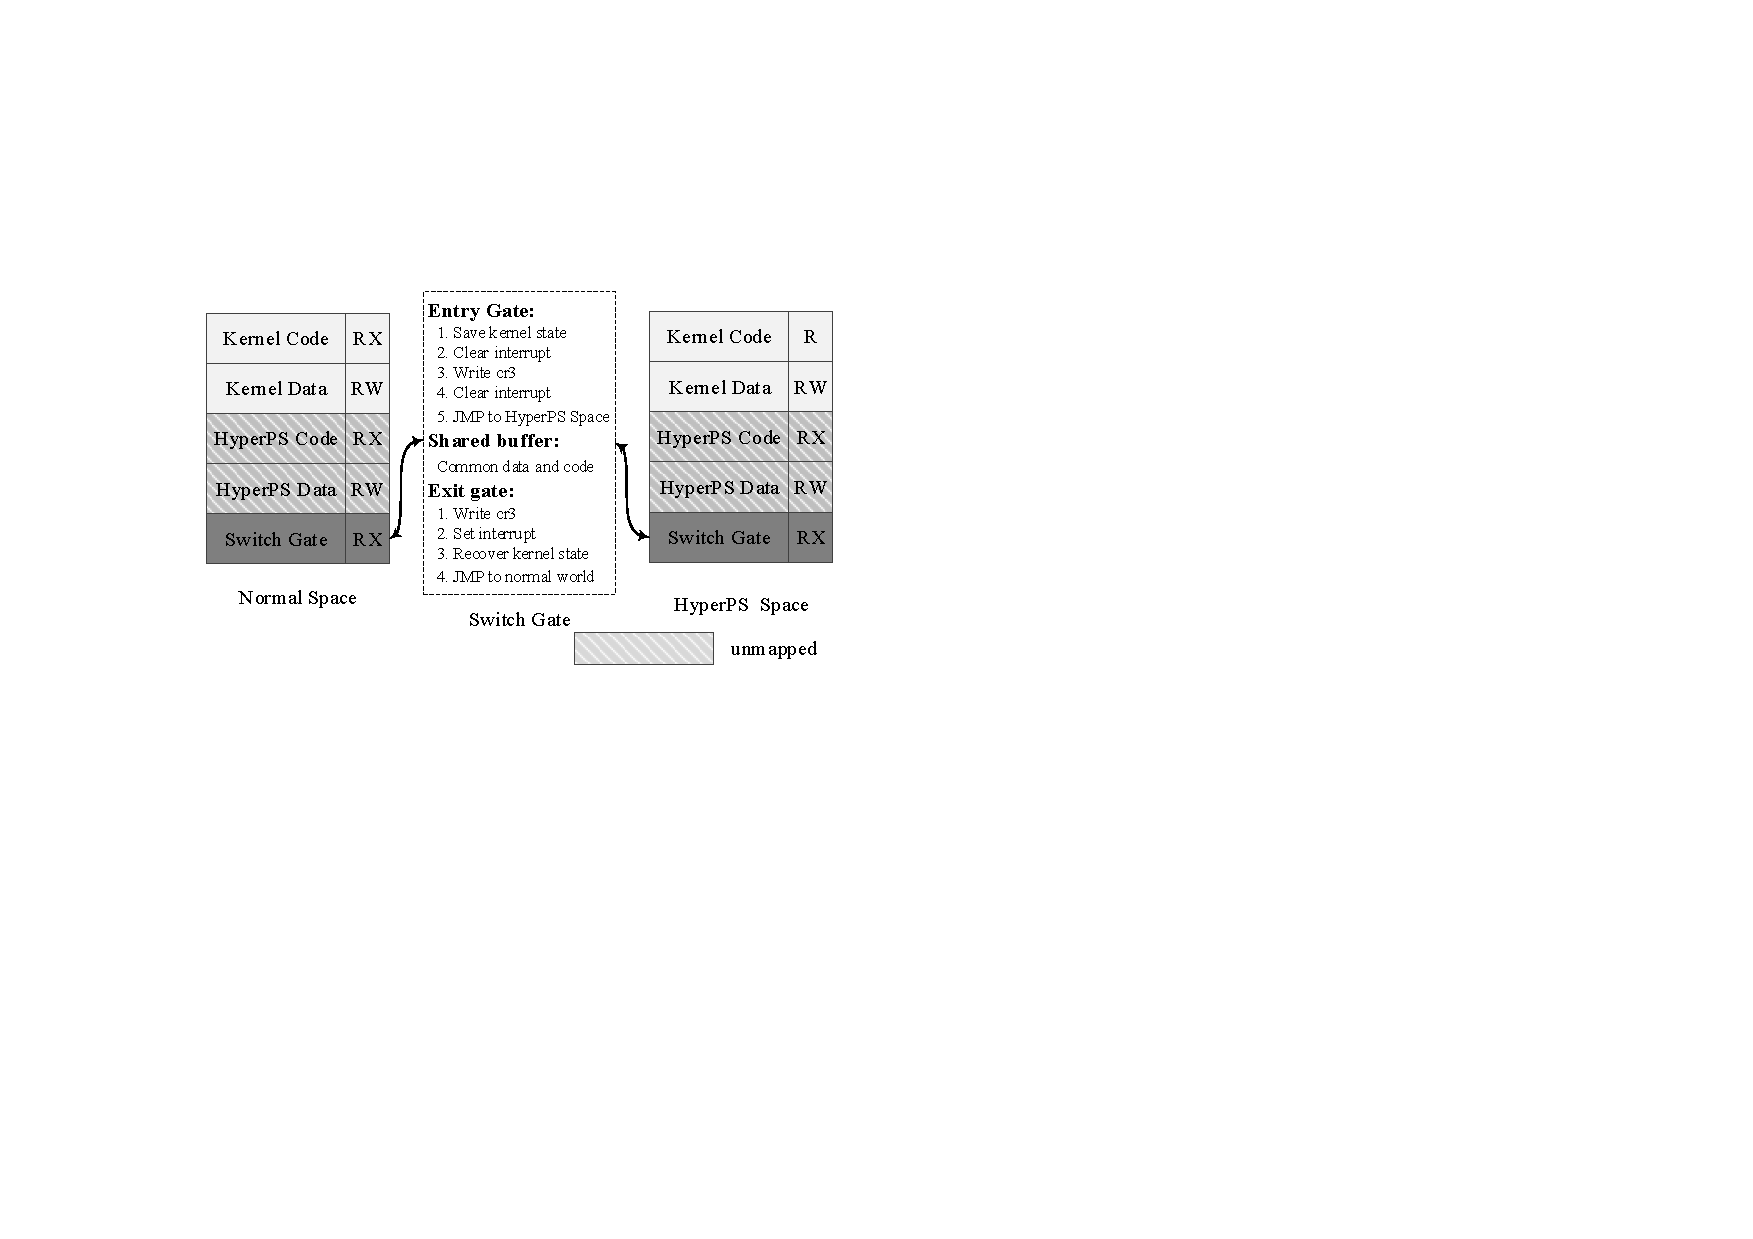
\includegraphics[width=0.8\linewidth]{IMG/address.pdf}
    \caption{Address layout of HyperPS}%
    \label{fig:address}
\end{figure}


% However,
% HyperPS Space的创建并不能在kernel boot阶段,因为此时,内核需要
% hostos的kernel并不能在boot的时候就直接完成两套页表的建立。
% As shown in this figure, HyperPS has to load itself into memory at first.
As shown in this figure, at the initialization stage, HyperPS has to load itself into memory firstly before it got executed. 
At this stage, all resources are managed by the Hostos kernel, HyperPS needs to request enormous numbers of memory allocation from the Hostos. These memories are used to hold HyperPS data and security tools that inherit compromised hypervisor's privileges of managing physical memory. 
In our prototype, we do not guarantee that all allocated memories are continuous in physical memory. 
Secondly, HyperPS creates a new page table that has already excluded the HyperPS Space. As shown in Figure \ref{fig:address}, this dedicated page table is placed in the Normal Space and accessed by the compromised HostOS kernel. 
Because all page table entries that are relative to HyperPS Space have been removed from that dedicated page table, 
% normal memory access beyond the HyperPS Space can not visit memory regions of HyperPS Space.
memory regions used by HyperPS are carved out of the memory ranges accessible to the HostOS kernel. 
% Thirdly, HyperPS will set a new GDT, IDT and stack for itself.
Thirdly, HyperPS returns execution back to the Normal Space by loading the address of the dedicated page table into the control register CR3. 
Forthly, as depicted in Figure \ref{fig:address}, we remove the execution bit in all kernel code (especially loadable kernel module code) entries of the page table used by HyperPS. 
HyperPS does not allow any execution of kernel code in the HyperPS Space in case attacker exploit kernel vulnerabilities in the HyperPS Space.
At last, we erase the page table entry that records the base address of the HyperPS page table.

On the execution of the three steps mentioned above, HyperPS has established an execution environment. 
However, at this time, this execution environment does not have the conditions for isolation and security, since the kernel can still modify this memory layout or access permission. 


\subsubsection{The Isolation of HyperPS Space}%
\label{ssub:the_isolation_of_hyperps_space}
% HyperPS has created a protected virtual address space.
HyperPS has to guarantee that the memory regions used by HyperPS are carved out of the memory ranges accessible to the kernel.
In order to achieve the isolation of the HyperPS Space, HyperPS restricts the compromised HostOS kernel access to this space. 
% To protect HyperPS Space, firstly, we deprive the write permission to whole kernel page tables,
Firstly, we removed write permissions to whole kernel page tables, so that the HostOS kernel can not modify the dedicated kernel page table in the Normal Space. In our prototype, the HostOS kernel can still navigate and examine page table entries, while write operations through legitimate page table management functions and macros are hooked and redirected into HyperPS Space. 
Meanwhile, direct write operations to the dedicated kernel page table will trigger an error (segment fault). 
% In our prototype, all page table write operations are completed inside the HyperPS Space.
% any modification operation will
% to
% navigation and examination of page table entries
% so that they are exclusively writable to HyperPS in the HyperPS Space.
% To protect HyperPS Space, write permission to HostOS kernel page tables
Secondly, as mentioned above, HyperPS removed all page table management functions and macros and replaced them with hooks that jump to HyperPS Space, so that any modification to the dedicated kernel page table in the Normal Space will be redirected to HyperPS Space. 
For example, \verb|native_set_pte()| is the function that actually implements PTE operations. Other PTE operation functions such as \verb|set_pte()| and \verb|native_set_pte_atomic()| all invoke the \verb|native_set_pte()| function to accomplish their implementation. 
% implement their
% will implement their operation by invoking this function.
In our prototype, HyperPS hooks all these final and elemental page table management functions and macros.
% For example, we hooked \verb|native_set_pte|, \verb|native_set_pmd| and \verb|do_page_fault|
HyperPS makes sure that the HostOS kernel can neither tamper the virtual memory permissions of the HyperPS Space, nor can it establish new mapping relationships to the physical memory frames related to the HyperPS Space. 
% For example,
In other word, the HostOS kernel page table is exclusively writable to HyperPS only. 
Lastly, HyperPS deprives the HostOS kernel of executing certain Control-Register-Relative functions so that it cannot direct the CPU to use alternative page tables other than the dedicated one we put in the Normal Space. 
% In this paper, HyperPS instrumented the kernel code to remove certain Control-Register-Relative functions.
For example, \verb|native_write_cr3()| is written with inline assembly language to load the page table's physical address into the register CR3. 
HyperPS instrumented this function to prevent the adversary from using an unverified page table. 
% HyperPS instrumented the function \verb|native_write_cr3| to prevent the adversary from using a unverified page table.
HyperPS also intercept the accessing operation to Control Register: CR0 to prevent the adversary from disabling the WP protection mechanism.
Actually, HyperPS hooked \verb|native_write_cr0()|, \verb|native_write_cr2()|, \verb|native_write_cr3()|, and \verb|native_write_cr4()| to HyperPS Space.
% redirect the execution to HyperPS Space.
% , such as the ones that change the vulue of CR0, CR3, and CR4.
By enforcing these three steps, the HostOS kernel running in the Normal Space can neither modify the dedicated host kernel page table nor change the control register configurations to use unverified page tables. 
As a result, the HostOS kernel cannot violate the isolation provided to HyperPS, since HyperPS deprives the HostOS kernel of privileges of accessing control registers and page tables and retains these privileges in the HyperPS Space.

% As a result, the HostOS kernel cannot violate the isolation provided to HyperPS, while HyperPS retains the exclusive access to control the control registers and page tables in the HyperPS Space.
% which
% is deprived the privileges of accessing to control registers and page tables in the HyperPS Space.
% retains the exclusive access to control the control registers and page tables in the HyperPS Space.



\iffalse
HyperPS makes sure that the HostOS kernel cannot modify any of the dedicated kernel page table to tamper the virtual memory access permissions of HyperPS Space. 

memory region used by HyperPS are carved out of the memory ranges accessible to the kernel.

In another word, the HostOS kernel page table are exclusively writable to HyperPS only. 


HyperPS will check 
so that the HostOS kernel is not allowed to change any ken
% Secondly, we also hook all page table management functions and macros to HyperPS Space, so that

. For example, we instrumented 

all page table functions 

这里HyperPS分为两步实现保护,一方面限制所有PT访问的函数。另外一方面限制CR3函数 

It starts by instrumenting the kernel code to remove certain MMU control instructions. such as the ones that change the location of memory tranlation tables. 
SEKK also monitor memory layout changes to guarantee that no other unverified privileged code is allowed to execute. 

hook的函数:
pte pme pagefualt 
vmcs read write clear 
pfn modify map 
clean page modify 
ksm page modify
\fi


\iffalse
下面的这部分内容应该是保护的内容,涉及的是EPT和缺页中断的处理,不应该是地址空间创建这部分内容。
在QEMU-KVM架构下,一台虚拟机的memory space同时受宿主机的page table和EPT两套页表管理。
% 在non-root模式下,
对于宿主机而言,虚拟机就是一个qemu进程,这个与其他的普通进程没有区别,宿主机通过传统的页表管理qemu所需要的所有地址空间。hostOS负责实际分配给该虚拟机的所有物理页框。
当EPT enable的时候,
在root模式下,EPT负责将qemu进程的

在QEMU-KVM架构下,以HostOS 视角看,整个虚拟机即为一个QEMU进程,EPT用于管理已经分配给QMEU进程中的物理页。
Traditional page tables continue to be reponsible for FVA-GPA, while EPT is responsible for GPA-HPA.
\fi

\iffalse
As shown in the Figure \ref{fig:address}, HyperPS creates the delicate kernel-level secure and isolated execution space by using two sets of page tables. 
On the left side of Figure \ref{fig:address}, the normal page table contains code and data of the HostOS kernel world. However, page table entries about the HyperPS Space has been removed from this table. %The attacker can not subvert the HyperPS Space 
Because all corresponding page table entries have been removed, the attacker can not find out in which memory the HyperPS Space locates, let alone subvert programs in the HyperPS Space. 
As shown in the Figure \ref{fig:address}, The Switch Gate is the only way that can perform the context switch from the Normal Space (the original hypervisor space) to the HyperPS Space.
On the other side of Figure \ref{fig:address}, HyperPS safeguard the integral page tables which contain both the kernel code, data and the HyperPS code, data. Besides, HyperPS removed the execution permission of all kernel code to prevent unauthorized code execution.
\fi

% \subsection{Switch Gate}
\subsection{Secure Switching}%
\label{sub:secure_switching}


Switch Gate is designed to allow secure switching between HyperPS Space and the Normal Space, and it is the only interface between the Normal Space and the HyperPS Space. In this paper, HyperPS adopts a technique similar to the one presented in SKEE \cite{azab2016skee}. Our Switch Gate can achieve atomic, deterministic and exclusive too.
% Switch Gate is the only interface between the Normal Space and the HyperPS Space. HyperPS adopts a technique similar to the one presented in SKEE \ref{Azab2016SKEE}. In this paper, our Switch Gate is designed to allow secure switching between HyperPS Space and the Normal Space. Our Switch Gate is designed to be atomic, deterministic and exclusive too.
As shown in the middle block of Figure \ref{fig:address}, the Switch Gate mainly consists of three parts: the Entry Gate, the Exit Gate and the Shared Buffer. 
The Entry Gate provides the only entrance for HyperPS Space. The Entry Gate will save the HostOS kernel state into the Shared Buffer first. Secondly, it will clear and disable interrupts. Interrupts could enable the compromised HostOS kernel to crash the atomic execution of Switch Gate. 
Then HyperPS will enter the HyperPS Space by loading the page table used by HyperPS Space into register Cr3. 
% load the page table used by HyperPS Space into register CR3.
The address of this page table is visible to HostOS kernel, however, as mentioned above, because all page table management functions and control register management functions have been hooked by HyperPS, the compromised HostOS kernel cannot subvert the HyperPS Space by using unverified page tables. 
Lastly, we clear interrupt with \verb|CLI| instruction again before we execute any instruction in the HyperPS Space. 
% divert execution into HyperPS Space.
The Exit Gate is the only interface that can divert execution back to Normal Space. It can only be invoked by HyperPS from the HyperPS Space. 
On receiving the invocation to Exit Gate, 
HyperPS will load the dedicated HostOS kernel page table into register CR3, recover interrupts and the saved kernel state. 
The Shared Buffer contains data and code shared by the Normal Space and the HyperPS Space. For example, as mentioned above, the entrance address of HyperPS Space and the return address to the Normal Space are stored in this buffer. HyperPS also stores the saved kernel state in this buffer. 
% In our prototype, we mapped the Switch Gate at the same place in both Normal Space and the HyperPS Space.

However, TLB becomes a subtle issue in the implementation of our Switch Gate. TLB is a special cache used to keep track of recently used PTE transactions.
Given a virtual address, the processor wll first examine the TLB if a PTE is present (TLB hit). If a match is found in the TLB, the processor retrieves the corresponding physical memory frame number from TLB directly. If the mapping is not cached by the TLB, the processor retrieves the physical memory page number from page table residing in the main memory and updates the new PTE into TLB. Thus, we need to flush TLB after we update both dedicated HostOS kernel page table and the page table used by HyperPS. 
In our prototype, we borrowed the idea in SecPod that clears the global bits in both the dedicated HostOS kernel page table and the HyperPS Space page table. By doing so, the TLB will always contain fresh address mappings after invoking the function \verb|flush_tlb_all()|.
% n HyperPS Space and

% there is one subtle issue in the implementation of the Switch Gate

% The switch gate is mapped at the same place in the Normal Space and the HyperPS Space, because the switch gate code must be called by the two worlds before and after switching. Of course, the entrance address must be protected after switching to HyperPS Space in case that a attacker accesses HyperPS Space causally after trusted boot. Protection to Switch Gate will be illustrated in the Section \ref{sec:securityforhyperps}.



% The shared buffer contains common data and code in Normal Space and the HyperPS Space. Common code is switch code, common data is entrance address to HyperPS Space and return address to the Normal World.
% On invoking Exit Gate,
% jump into
%  before
% address of page table

% HyperPS achieves the atomic secure switching
% Disabling interrupts
% 为什么要屏蔽中断,这里要说清除。

\iffalse
In the middle of Figure \ref{fig:address}, the switch gate includes entry/exit gate and shared buffer. Entry gate provides the only entrance to HyperPS Space and the exit gate provides the address for returning to the Normal Space. The shared buffer contains common data and code in Normal Space and the HyperPS Space. Common code is switch code, common data is entrance address to HyperPS Space and return address to the Normal World. The switch gate is mapped at the same place in the Normal Space and the HyperPS Space, because the switch gate code must be called by the two worlds before and after switching. Of course, the entrance address must be protected after switching to HyperPS Space in case that a attacker accesses HyperPS Space causally after trusted boot. Protection to Switch Gate will be illustrated in the Section \ref{sec:securityforhyperps}.
%添加Section的引用
\fi

\iffalse
except for that of HyperMI World. This can prevent compromised hypervisor from breaking the integrity of HyperMI World. Programs running in normal world can not access data in HyperMI World. On the right of Figure \ref{fig2}, all address is mapped in HyperMI page table.

 We use two isolated address spaces based on two sets of page tables to achieve isolation of HyperMI World.
Figure \ref{fig2} describes the address space layout of two worlds through two sets of page table, the normal page table and HyperMI page table. On the left of Figure \ref{fig2}, the normal page table contains code and data of the normal world except for that of HyperMI World. This can prevent compromised hypervisor from breaking the integrity of HyperMI World. Programs running in normal world can not access data in HyperMI World. On the right of Figure \ref{fig2}, all address is mapped in HyperMI page table.
HyperMI code remains executable and HyperMI data remains writable. What's the most important, kernel code is forbid to execute when HyperMI World is active, so that it can not attack HyperMI World.

\textbf{Creating Switch Gate}
In the middle of Figure \ref{fig2}, the switch gate includes entry/exit gate and shared buffer. Entry gate provides the only entrance to HyperMI World and the exit gate provides the address for returning to the normal world. The shared buffer contains common data and code in normal world and HyperMI World. Common code is switch code, common data is entrance address to HyperMI World and return address to the normal world. The switch gate is mapped at the same place in the normal world and HyperMI World because the switch gate code must be called by the two worlds before and after switching. Of course, the entrance address must be protected after switching to HyperMI World in case that a attacker accesses HyperMI World causally after trusted boot. This is introduced in section \ref{SG}.
\fi





\iffalse
下面的这部分内容应该是保护的内容,涉及的是EPT和缺页中断的处理,不应该是地址空间创建这部分内容。
在QEMU-KVM架构下,一台虚拟机的memory space同时受宿主机的page table和EPT两套页表管理。
% 在non-root模式下,
对于宿主机而言,虚拟机就是一个qemu进程,这个与其他的普通进程没有区别,宿主机通过传统的页表管理qemu所需要的所有地址空间。hostOS负责实际分配给该虚拟机的所有物理页框。
当EPT enable的时候,
在root模式下,EPT负责将qemu进程的

在QEMU-KVM架构下,以HostOS 视角看,整个虚拟机即为一个QEMU进程,EPT用于管理已经分配给QMEU进程中的物理页。
Traditional page tables continue to be reponsible for FVA-GPA, while EPT is responsible for GPA-HPA.
\fi


\iffalse
###################
三个章节的内容
KVM 函数hook 
EPT处理流程
KSM是特别要处理的内容
###################
\fi

\subsection{Privilege Deprivation and Management}%
\label{sub:privilege_deprivation_and_management}


In HyperPS, the HostOS has been deprived of the privileges of managing physical memory. This gives HyperPS complete control over the guest VM's virtual-physical memory mapping and protection. In our prototype, we hook all KVM's VMX and EPT functions to redirect EPT management to our HyperPS Space.

% TODO 上面说要保护管理EPT,但是这里为什么要从VMCS入手,这里要说明
\subsubsection{VMCS Hook}%
\label{ssub:vmcs_hook}


Based on Intel manuals, VMCS can only be manipulated by several privileged instructions: \verb|VMPTRLD|, \verb|VMCLEAR| \verb|VMPTRLD|, \verb|VMREAD|, \verb|VMWRITE|, \verb|VMLAUNCH|, and so on.
In the QEMU-KVM architecture, the KVM provides a wrapper around these privileged instructions. The QEMU does not need to deal architecture specific details, it just needs to invoke the wrapper functions in KVM with proper parameters.
% the KVM is responsible for executing these privileged instructions. The KVM provides a wrapper around these privileged instructions. The QEMU does not need to deal architecture specific details, it just need to invoke KVM functions with proper parameters.
In Linux, all VMX operation functions are defined in the file \verb|vmx_ops.h|. 
For example, \verb|vmcs_writel()| wraps the privileged instruction \verb|VMWRITE|, it will update the specified field of a VMCS with a given value. 
% the value to a VMCS filed
\verb|__vmcs_readl()| is one of wrapper functions to the privileged instruction \verb|VMREAD|, this function reads a field from a VMCS and returns field value. 
% it into
In our prototype, we implement all VMX functions in Normal Space with hooks to HyperPS Space to provide all VMX services. 
In particular, we prevent the HostOS/Hypervisor from loading an unverified EPTP. 
HyperPS interposes the execution of \verb|vmcs_writel()|, and the Context Management in the HyperPS Space Management component checks the invoked parameters and verifies if the write to \verb|VM-Execution Control Fields.EPTP| is legal or not. 
HyperPS also forbids arbitrary write to the \verb|VM-Function Controls| field in \verb|VM-Execution Control Fields|.
The field \verb|VM-Function Controls| contains the physical address of the 4-KByte EPTP list. Invalid value in the EPTP list may lead to an unverified EPTP value. 

\subsubsection{EPT Hook}%
\label{ssub:ept_hook}


In this paper, because EPTs have been removed from the Normal Space, 
HyperPS needs to hooks EPT functions that access EPTP and EPT Paging Structures to HyperPS Space, and implement these services in the HyperPS Space.
In QEMU-KVM architecture, the KVM is the component that maintains EPTs, while QEMU is responsible for requesting memory allocation.
Thus, in our prototype, we dig into KVM to find out all functions that process EPTPs and EPTs directly. Figure \ref{fig:impept} depicts how HyperPS handles all EPT management functions. 

\begin{figure}[htpb]
    \centering
    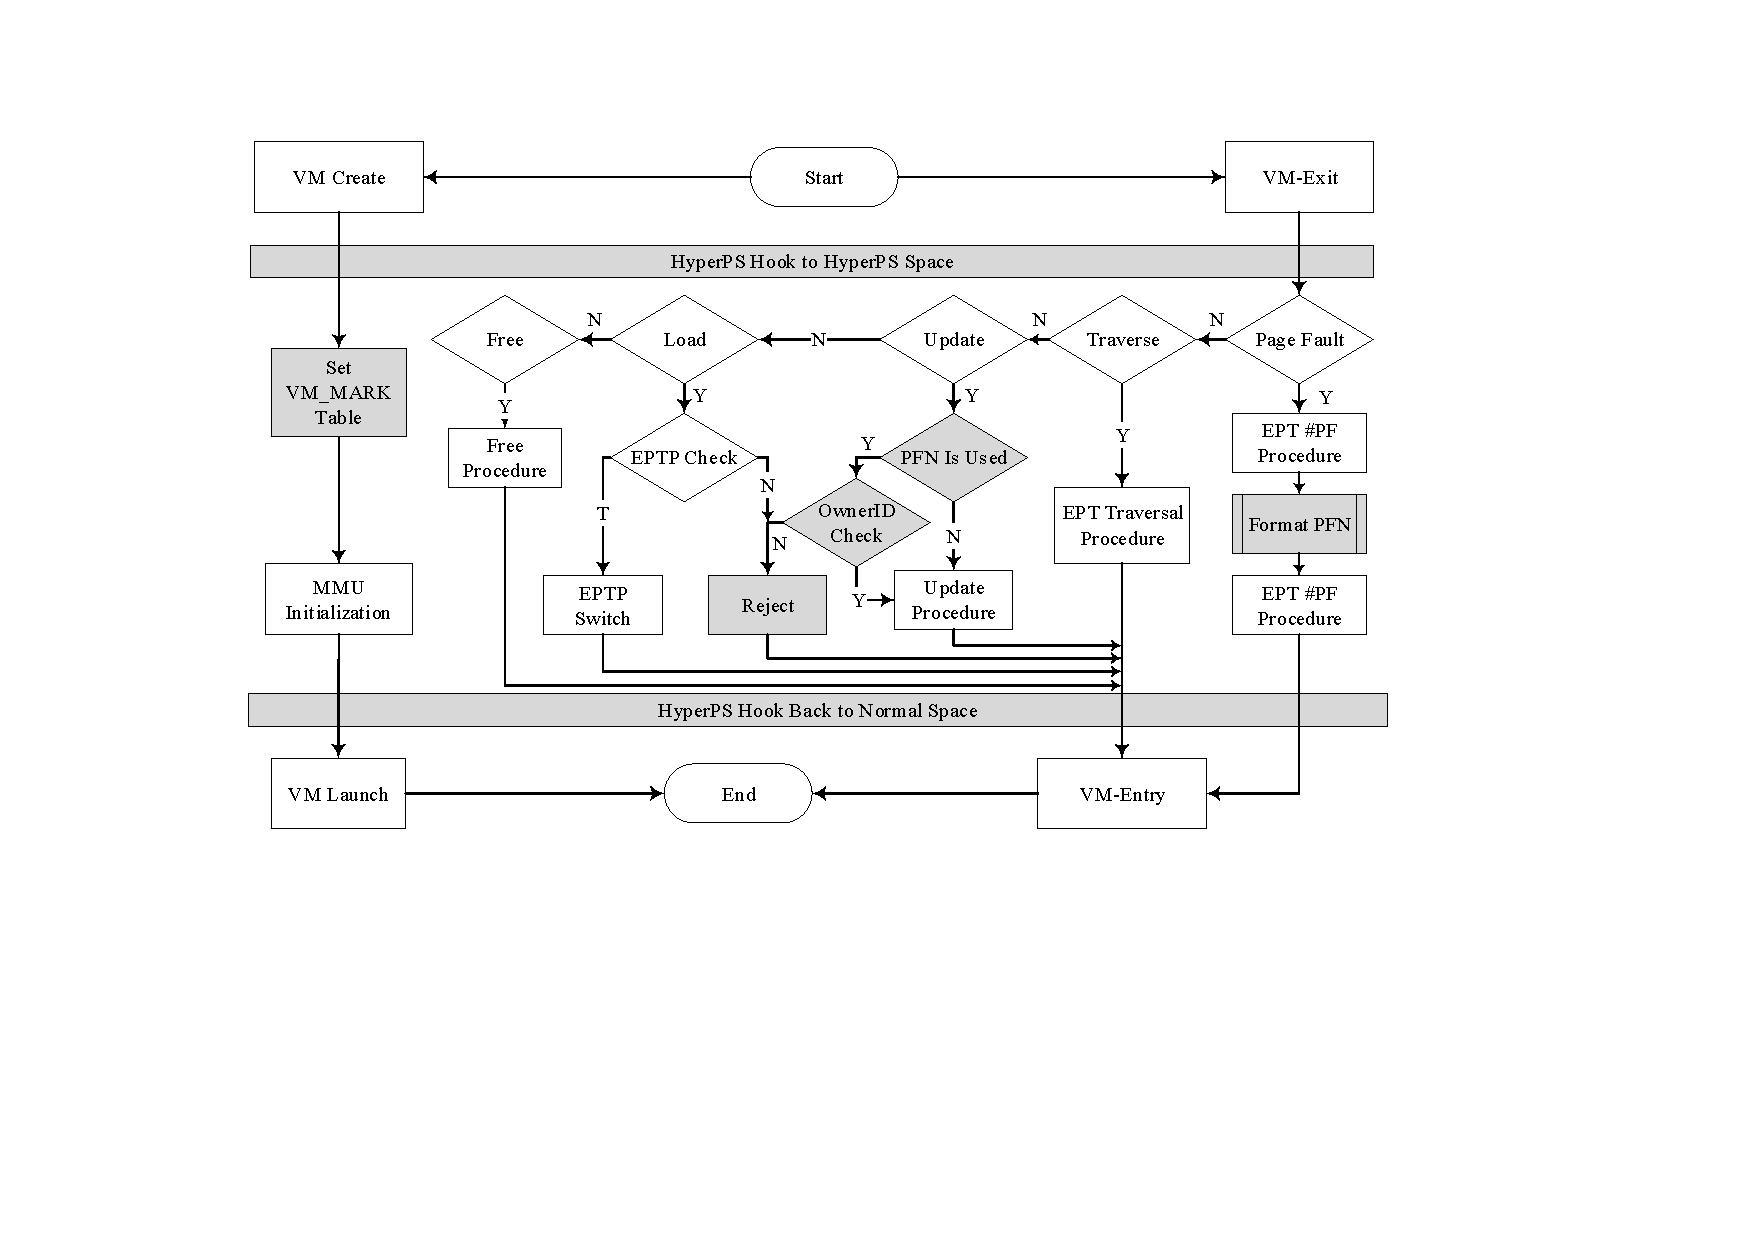
\includegraphics[width=1\linewidth]{./IMG/imp-ept-handle.pdf}
    \caption{HyperPS EPT Procedure}%
    \label{fig:impept}
\end{figure}

% MMU Initialization:
\textbf{EPT Creation}: The KVM will create and initialize MMU along with the creation of vcpu. 
If the EPT is supported and enabled by the hardware, The KVM module will invoke the function \verb|init_kvm_tdp_mmu| to initialize the MMU. 
Actually, the function \verb|init_kvm_tdp_mmu()| is just responsible for registering all kinds of EPT management functions to the inputted vcpu management structure: \verb|vcpu->arch.mmu|. 
For example, the EPT page fault function is initialized to \verb|kvm_tdp_page_fault()|, meanwhile inject page fault function is initialized to \verb|kvm_inject_page_fault()|. 
In our prototype, we hooked all these registered functions into HyperPS Space. However, it is far from sufficient to hook these functions only. We need to dig into the internal of these functions to find out all surplus functions that access VMCS or EPT directly.

Besides, in this paper, we implement a new structure VM-Mark Table to guarantee the legitimate relationship between the VM and the EPT. 
During the creation of EPT, the function \verb|vmx_load_mmu_pgd()| is responsible for writing the newly created EPTP to the corresponding VMCS.
In our prototype, as shown in Figure \ref{fig:impept}, we hooked this function into the HyperPS Space. In the HyperPS Space, we also implemented our protection that stores and synchronizes the corresponding EPTP value and VM identifier to VM-Mark Table. 


% we also hooked the function \verb|vmx_load_mmu_pgd()|, which will write the new created EPTP to the corresponding VMCS.
% In our prototype, as shown in Figure \ref{fig:impept}, we will store and synchronize the corresponding EPTP value and VM identifier to VM-Mark Table.
% guarantee that only legitimate EPTP can be loaded
% Actually, the \verb|init_kvm_tdp_mmu()| just registers lots of exception handling functions, such as \verb|kvm_tdp_page_fault()| to a stucture \verb|vcpu->arch.mmu|.
% If the EPT is supported, the function \verb|init_kvm_tdp_mmu| is responsible for initializing the MMU.
\iffalse
Runtime EPT Management: 
As shown in Figure \ref{fig:impept}, we classified all EPT management operations into five types: Page Fault, Update, Traverse, Load and Free. 
In our prototype, because EPT and EPTP have been removed from the Normal Space, we have to hook all these functions into the HyperPS Space and implement  the respective EPT access services in the HyperPS Space. 
\fi

% EPT Construction Process:
\textbf{EPT Page fault}:
The KVM adopts a similar page table construction process to the kernel page table that fills EPT paging structures by handling EPT page fault. 
As mentioned above, if the EPT page fault occurs, the KVM invokes the function \verb|kvm_tdp_page_fault()| to handle this exception. 
% As mentioned above, the KVM invokes the function \verb|kvm_tdp_page_fault()| to handle EPT page fault.
Typically, the KVM is not responsible for the allocation of physical pages. 
It is responsible for synchronizing the allocated physical page frame number (PFN) to the corresponding EPT Paging-structure. We classify EPT operations in EPT Page Fault into Update. 
% What KVM does is to synchronize the allocated physical page frame number (PFN) to the corresponding EPT paging-structure. We classify EPT operations in EPT Page Fault into Update.
In a virtualization environment, there is a memory reclamation technique, called Ballooning, that is used by the hypervisor to allow the physical host system to retrieve memories from certain guest virtual machine and share them with others. 
However, Ballooning may be abused to facilitate side channel attacks. 
In this paper, we take such kind of situation into consideration. As depicted in Figure ref{fig:impept}, 
HyperPS will format the allocated physical memory frame before mapping it in the EPT while executing the function \verb|kvm_tdp_page_fault()|. More details are illustrated in Section \ref{sub:ksm_handle}. 
% TODO 添加章节的引用
% we hook the function \verb|kvm_tdp_page_fault()| into HyperPS Space, and format the allocated physical memory frame before mapping it in the EPT in this function.
% HyperPS will formate the
% different virtual machines shared the same physical memory.

\textbf{EPT Traverse}: 
% Though HyperPS does not interpose the traversal of EPT,
Because all EPTs have been moved from the Normal Space to the HyperPS Space, though HyperPS does not interpose the traversal of EPT, HyperPS also needs to instrument EPT traversal functions, so that they can access EPTs. 
However, we do not need to re-implement EPT traversal services in the HyperPS Space. In our prototype, we just implement a hook function that will invoke the Switch Gate to retrieve the corresponding EPTP value or EPT Paging Structure value. 
For example, the function \verb|shadow_walk_init()| is responsible for initializing the structure \verb|kvm_shadow_walk_iterator| structure which will record the value of EPTP and be used in the traversal of EPTs. We added the hook function inside the function \verb|shadow_walk_init()| to access EPT in HyperPS Space. 

\textbf{EPT Load}: 
In this paper, we propose a VM-Mark table to tag the mapping relations between the EPT and the corresponding virtual machine. 
HyperPS will be engaged to check whether the loaded EPT corresponds to the virtual machine every time the virtual is going to executing VM-Entry. 
\verb|vcpu_enter_guest()| is an arch-specific function in KVM to start up a virtual machine. 
As depicted in Figure \ref{fig:impept}, we placed a hook before executing the function \verb|vmx_load_mmu_pgd()| inside this function. The function \verb|vmx_load_mmu_pgd()| is the final function that load the EPT. 
If the EPTP (the base address of the EPT) matches an item in the VM-Mark Table, HyperPS will allow the subsequent operations, such as EPTP Switch and EPT Load. Otherwise, HyperPS will terminate the execution of the corresponding virtual machine. 

\textbf{EPT Update}: 
In this paper, we propose a new structure: Page-Mark Table to record the relationships between EPT Paging-structures and the physical memory page frames. 
HyperPS guarantees that physical page frames with write permission can only be accessed with one determinate VM. 
Physical page frames shared by different machines can only be read-only. 
Besides, HyperPS guarantees that virtual machines participating the memory sharing are authenticated and recorded by us. 
Figure \ref{fig:impept} depicts the rough process of how HyperPS handles EPT Update. 
As mentioned above, in this paper, in addition to changing the permissions of EPT entries, HyperPS also regards the allocation of a new EPT Paging-structure as EPT Update. 
In our prototype, we do not get involved in new physical memory page frame allocation. We focus on operations to EPTs only. 
The function \verb|__direct_map()| in KVM is the core function to build new EPT entries. HyperPS places hooks inside this function to perfrom security checks. If the allocated physical frame number is untracked in the Page-Mark Table, HyperPS will first invokes the function mentioned above to format this allocated physical page. Then, HyperPS hooks the function \verb|kvm_mmu_get_page()|, the function \verb|link_shadow_page()|, and the function \verb|mmu_set_spte()| into the HyperPS Space.
In the HyperPS Space, HyperPS will initialize a new EPT Paging-structure, and link it to the EPT.
% and link it to the corresponding

\iffalse
access to one VM or shared with
the effective isolation between diffe
In this paper, we define EPT Update as assigning a new EPT paging-structure or updating EPT paging-structures. 
\verb|__direct_map()| is the core function to build the page table.
\verb|kvm_mmu_get_page()| 分配一个EPT 页表项 
\verb|link_shadow_page()| 将新分配到下一级页表页的基地址填充到当前页表项SPTE中

\verb|mmu_set_spte| is the final calling function to set the page table structure. 
\fi

\iffalse
if the the EPT and the 
every time a virtual machine is going to be loaded into Non-Root model. 
\verb|vcpu_enter_guest()| is an arch-specific function in KVM to start up a virtual machine. 
In this function, we placed a hook before executing the function \verb|vmx_load_mmu_pgd()| inside this function. 
This function will will invoke the function \verb|vmx_load_mmu_pgd()| to load the EPT. 
The KVM will invoke the function \verb|vcpu_enter_guest()| to 
to load the corresponding EPT 
Every time the virtual machine runs, execute \verb|vcpu_enter_guest()|, this function load EPT.
EPT traversal functions in HyperPS Space.
In our prototype, we do not re-implement all EPT traversal functions in HyperPS Space, but just implement a hook function to retrieve
to hook these EPT traversal functions. 
In our prototype, we 
The structure \verb|kvm_shadow_walk_iterator| is the most important structure used in the traversal of the EPT. 
This structure records the value of EPTP. 
% In our prototype,


When Guest Address has EPT Violation, KVM uses \verb|kvm_shadow_walk_iterator| to complete the traversal of the EPT, look up the page table entry EPT corresponding to Guest Address step by step, and finally index to the corresponding page table entry in the leaf page table to get the Guest Address corresponding the number of the page frame.
The function \verb|shadow_walk_init()| takes the physical address of the guest where the EPT Violation occurred and the VCPU with EPT Violation as input. 
This function is responsible for initializing the struct \verb|kvm_shadow_walk_iterator| structure, preparing to traverse the EPT page table.

In this paper, HyperPS does not hook EPT traversal functions, such as data structure \verb|kvm_shadow_walk_iterator()| in KVM. 
\verb|kvm_walk_init_using_root()| takes \verb|kvm_shadow_walk_iterator| as input. 
\verb|shadow_walk_okay()| \verb|shadow_walk_next()|

\verb|kvm_shadow_walk_iterator| records the value of EPTP
\fi
% It just maintains EPTs. Thus,
% what the KVM does in Page Fault Handling is similar to
% As shown in Figure \ref{fig:impept}, we interfere in the EPT
% The EPT paging structures are also completed by handing page fault exceptions.
% the KVM is not responsible for the allocation of physical pages. It just maintains EPTs.
% Memory allocation are completed with QEMU and the HostOS Kernel.
% after the QEMU requested allocation
\iffalse
\verb|__direct_map()| is the core function to build the page table.
\verb|kvm_mmu_get_page()| 分配一个EPT 页表项 
\verb|link_shadow_page()| 将新分配到下一级页表页的基地址填充到当前页表项SPTE中

\verb|mmu_set_spte| is the final calling function to set the page table structure. 

HyperPS needs to hooks all EPT management function in the Normal Space to HyperPS Space. 
EPT Creation: 
% we hooked all EPT management operation functions.

If the EPT is supported, the function \verb|init_kvm_tdp_mmu| is responsible for initalizing the MMU. 

Though HyperPS does not interpose the traversal of EPT, Because all EPTs have been moved from the Normal Space to the HyperPS Space, HyperPS also need to hook these EPT traversal functions. 

When Guest Address has EPT Violation, KVM uses \verb|kvm_shadow_walk_iterator| to complete the traversal of the EPT, look up the page table entry EPT corresponding to Guest Address step by step, and finally index to the corresponding page table entry in the leaf page table to get the Guest Address corresponding the number of the page frame.
The function \verb|shadow_walk_init()| takes the physical address of the guest where the EPT Violation occurred and the VCPU with EPT Violation as input. 
This function is responsible for initializing the struct \verb|kvm_shadow_walk_iterator| structure, preparing to traverse the EPT page table.

In this paper, HyperPS does not hook EPT traversal functions, such as data structure \verb|kvm_shadow_walk_iterator()| in KVM. 
\verb|kvm_walk_init_using_root()| takes \verb|kvm_shadow_walk_iterator| as input. 
\verb|shadow_walk_okay()| \verb|shadow_walk_next()|

\verb|kvm_shadow_walk_iterator| records the value of EPTP

every time the virtual machine runs, execute \verb|vcpu_enter_guest()|, this function load EPT.

transfer \verb|kvm_mmu_load()| set customer CR3

KVM is not responsible for the allocation of physical pages, but maintains EPT. 

\verb|hva_to_pfn()|: get the host physical page frame number from the host vurtual address.

\verb|__direct_map()| is the core function to build the page table.
\verb|kvm_mmu_get_page()| 分配一个EPT 页表项 
\verb|link_shadow_page()| 将新分配到下一级页表页的基地址填充到当前页表项SPTE中

\verb|mmu_set_spte| is the final calling function to set the page table structure. 

when the page is invalid, it will eventually call \verb|kvm_mmu_free_page()| recycling, here is mainly to see when it will be recycled
when EPT is loaded, \verb|mmu_load_direct_root()| \verb|make_mmu_page_available|.
\fi

% which will crash
% HyperPS instrumented this function to prevnet the adversary from using a unverified page table.
% the respective hooked functions
% HyperPS hooks these functions into the HyperPS Space. In the HyperPS Space, Context Management in the HyperPS Space Management component check the invoked parameters and verifies if the write to \verb|VM-Execution Control Fields.EPTP| is legal or not.
\iffalse

\subsection{KSM Handle}\label{ssub:ksm_handle}
%{}. 
% TODO 添加章节的引用
% we hook the function \verb|kvm_tdp_page_fault()| into HyperPS Space, and format the allocated physical memory frame before mapping it in the EPT in this function.
% HyperPS will formate the
% different virtual machines shared the same physical memory.

\textbf{EPT Traverse}: 
% Though HyperPS does not interpose the traversal of EPT,
Because all EPTs have been moved from the Normal Space to the HyperPS Space, though HyperPS does not interpose the traversal of EPT, HyperPS also need to instrument EPT traversal functions, so that they can access EPTs. 
However, we do not need to re-implement EPT traversal services in the HyperPS Space. In our prototype, we just implement a hook function that will invokes the Switch Gate to retrieve the corresponding EPTP value or EPT Paging Structure value. 
For example, the function \verb|shadow_walk_init()| is responsible for initializing the structure \verb|kvm_shadow_walk_iterator| structure which will record the value of EPTP and be used in the traversal of EPTs. We added the hook functions inside the function \verb|shadow_walk_init()| to access EPT in HyperPS Space. 

\textbf{EPT Load}: 
In this paper, we propose a VM-Mark table to tag the mapping relations between the EPT and the corresponding virtual machine. 
HyperPS will be engaged to check whether the loaded EPT corresponds to the virtual machine at every time the virtual is going to executing VM-Entry. 
\verb|vcpu_enter_guest()| is an arch-specific function in KVM to start up a virtual machine. 
As depicted in Figure \ref{fig:impept}, we placed a hook before executing the function \verb|vmx_load_mmu_pgd()| inside this function. The function \verb|vmx_load_mmu_pgd()| is the final function that load the EPT. 
If the EPTP (the base address of the EPT) matches an item in the VM-Mark Table, HyperPS will allow the subsequent operations, such as EPTP Switch and EPT Load, otherwise HyperPS will terminate the execution of the corresponding virtual machine. 

\textbf{EPT Update}: 
In this paper, we propose a new structure: Page-Mark Table to record the relationships between EPT paging-structures and the physical memory page frames. 
HyperPS guarantees that physical page frame with write permission can only be accessed with one determinate VM. 
Physical page frames shared by different machines can only be read-only. 
Besides, HyperPS guarantees that virtual machines participating the memory sharing are authenticated and recorded by us. 
Figure \ref{fig:impept} depicts the rough process of how HyperPS handles EPT Update. 
As mentioned above, in this paper, in addition to changing the permissions of EPT entries, HyperPS also regards the allocation of a new EPT paging-structure as EPT Update. 
In our prototype, we do not get involved in new physical memory page frame allocation, we focus on operations to EPTs only. 
The function \verb|__direct_map()| in KVM is the core function to build new EPT entries. HyperPS places hooks inside this function to perfrom security checks. If the allocated physical frame number is untracked in the Page-Mark Table, HyperPS will first invokes the function mentioned above to format this allocated physical page. Then, HyperPS hooks the function \verb|kvm_mmu_get_page()|, the function \verb|link_shadow_page()|, and the function \verb|mmu_set_spte()| into the HyperPS Space.
In the HyperPS Space, HyperPS will initialize a new EPT paging-structure, and link it the EPT.
% and link it to the corresponding
\fi

\iffalse
access to one VM or shared with
the effective isolation between diffe
In this paper, we define EPT Update as assigning a new EPT paging-structure or updating EPT paging-structures. 
\verb|__direct_map()| is the core function to build the page table.
\verb|kvm_mmu_get_page()| 分配一个EPT 页表项 
\verb|link_shadow_page()| 将新分配到下一级页表页的基地址填充到当前页表项SPTE中

\verb|mmu_set_spte| is the final calling function to set the page table structure. 
\fi

\iffalse
if the the EPT and the 
every time a virtual machine is going to be loaded into Non-Root model. 
\verb|vcpu_enter_guest()| is an arch-specific function in KVM to start up a virtual machine. 
In this function, we placed a hook before executing the function \verb|vmx_load_mmu_pgd()| inside this function. 
This function will will invoke the function \verb|vmx_load_mmu_pgd()| to load the EPT. 
The KVM will invoke the function \verb|vcpu_enter_guest()| to 
to load the corresponding EPT 
Every time the virtual machine runs, execute \verb|vcpu_enter_guest()|, this function load EPT.
EPT traversal functions in HyperPS Space.
In our prototype, we do not re-implement all EPT traversal functions in HyperPS Space, but just implement a hook function to retrieve
to hook these EPT traversal functions. 
In our prototype, we 
The stucture \verb|kvm_shadow_walk_iterator| is the most important structure used in the traversal of the EPT. 
This structure recordes the value of EPTP. 
% In our prototype,


When Guest Address has EPT Violation, KVM uses \verb|kvm_shadow_walk_iterator| to complete the traversal of the EPT, look up the page table entry EPT corresponding to Guest Address step by step, and finally index to the corresponding page table entry in the leaf page table to get the Guest Address corresponding the number of the page frame.
The function \verb|shadow_walk_init()| takes the physical address of the guest where the EPT Violation occurred and the VCPU with EPT Violation as input. 
This function is responsible for initializing the struct \verb|kvm_shadow_walk_iterator| structure, preparing to traverse the EPT page table.

In this paper, HyperPS does not hook EPT traversal functions, such as data structure \verb|kvm_shadow_walk_iterator()| in KVM. 
\verb|kvm_walk_init_using_root()| takes \verb|kvm_shadow_walk_iterator| as input. 
\verb|shadow_walk_okay()| \verb|shadow_walk_next()|

\verb|kvm_shadow_walk_iterator| records the value of EPTP
\fi
% It just maintains EPTs. Thus,
% what the KVM does in Page Fault Handling is similar to
% As shown in Figure \ref{fig:impept}, we interfere in the EPT
% The EPT paging structures are also completed by handing page fault exceptions.
% the KVM is not responsible for the allocation of physical pages. It just maintains EPTs.
% Memory allocation are completed with QEMU and the HostOS Kernel.
% after the QEMU requested allocation
\iffalse
\verb|__direct_map()| is the core function to build the page table.
\verb|kvm_mmu_get_page()| 分配一个EPT 页表项 
\verb|link_shadow_page()| 将新分配到下一级页表页的基地址填充到当前页表项SPTE中

\verb|mmu_set_spte| is the final calling function to set the page table structure. 

HyperPS needs to hooks all EPT management function in the Normal Space to HyperPS Space. 
EPT Creation: 
% we hooked all EPT management operation functions.

If the EPT is supported, the function \verb|init_kvm_tdp_mmu| is responsible for initalizing the MMU. 

Though HyperPS does not interpose the traversal of EPT, Because all EPTs have been moved from the Normal Space to the HyperPS Space, HyperPS also need to hook these EPT traversal functions. 

When Guest Address has EPT Violation, KVM uses \verb|kvm_shadow_walk_iterator| to complete the traversal of the EPT, look up the page table entry EPT corresponding to Guest Address step by step, and finally index to the corresponding page table entry in the leaf page table to get the Guest Address corresponding the number of the page frame.
The function \verb|shadow_walk_init()| takes the physical address of the guest where the EPT Violation occurred and the VCPU with EPT Violation as input. 
This function is responsible for initializing the struct \verb|kvm_shadow_walk_iterator| structure, preparing to traverse the EPT page table.

In this paper, HyperPS does not hook EPT traversal functions, such as data structure \verb|kvm_shadow_walk_iterator()| in KVM. 
\verb|kvm_walk_init_using_root()| takes \verb|kvm_shadow_walk_iterator| as input. 
\verb|shadow_walk_okay()| \verb|shadow_walk_next()|

\verb|kvm_shadow_walk_iterator| records the value of EPTP

every time the virtual machine runs, execute \verb|vcpu_enter_guest()|, this function load EPT.

transfer \verb|kvm_mmu_load()| set customer CR3

KVM is not responsible for the allocation of physical pages, but maintains EPT. 

\verb|hva_to_pfn()|: get the host physical page frame number from the host vurtual address.

\verb|__direct_map()| is the core function to build the page table.
\verb|kvm_mmu_get_page()| 分配一个EPT 页表项 
\verb|link_shadow_page()| 将新分配到下一级页表页的基地址填充到当前页表项SPTE中

\verb|mmu_set_spte| is the final calling function to set the page table structure. 

when the page is invalid, it will eventually call \verb|kvm_mmu_free_page()| recycling, here is mainly to see when it will be recycled
when EPT is loaded, \verb|mmu_load_direct_root()| \verb|make_mmu_page_available|.
\fi

% which will crash
% HyperPS instrumented this function to prevnet the adversary from using a unverified page table.
% the respective hooked functions
% HyperPS hooks these functions into the HyperPS Space. In the HyperPS Space, Context Management in the HyperPS Space Management component check the invoked parameters and verifies if the write to \verb|VM-Execution Control Fields.EPTP| is legal or not.


\subsection{KSM Handle}%
\label{sub:ksm_handle}
Kernel Same-page Merging (KSM), used by the KVM Hypervisor, allows KVM guests to share identical memory pages. 
KSM enables the KVM Hypervisor to examine two or more already running virtual machines and compare their memory. If any memory region or pages are identical, KSM reduces multiple identical memory pages to a single page. 
% This merged page is marked Copy-On-Write (COW). If the contents of the page is modified by a guest virtual machine, a new page is created for that guest.
The KSM adopts two red-black trees: the unstable tree and the stable tree, to implement its service.
The unstable tree holds pointers to pages that have been found to be unchanged for a period of time. 
The stable tree holds pointers to all the merged pages (KSM pages), sorted by their contents. All pages in the stable tree are write-protected. 
If the contents of the page is modified by a guest virtual machine, a new page is created for that guest.
Once a merged page has been recorded into the stable tree, the merged page pointer will never be removed from the stable tree until all users have either modified or unmapped it. 
At runtime, for each page scanned, the KSM proceeds to search a match first in the stable tree that only contains already shared pages. If a match is found in the stable tree, KSM will merge this scanned page with the KSM page found in the stable. 
If no match is found in the stable tree, KSM will then search the unstable tree. If a match is found in the unstable tree, the page is merged with the page in the unstable tree, and the resulting KSM merged page is added to the stable tree. 

In this paper, as mentioned in Section \ref{ssub:ept_paging_structure_protection}, we also take KSM into consideration. 
\verb|stable_tree_insert()|, \verb|stable_tree_append()| are the functions in KSM to add the merged page into stable tree. 
Firstly, As mentioned above, we placed hooks in these stable tree operation functions to trap execution to HyperPS Space. 
In our prototype, the Page-Mark Table is used to record all physical page frames used by the VM. If a page is merged by KSM, HyperPS fills the \verb|SharedID| with the corresponding VM identifier. 
Secondly, Merging page results in EPT update too. HyperPS needs to get involved in the page merging process too. 
\verb|try_to_merge_one_page()| and \verb|try_to_merge_two_page()| are the function in KSM to merge two pages into one. 
For EPTs have been moved to HyperPS Space and EPT management functions are hooked to HyperPS Space too, we also hook these functions to HyperPS Space to synchronize the memory mapping changes to EPT.

\iffalse
Page-Mark Table is 
HyperPS will record
We present the field \verb|SharedID| in the Page-Mark Structure to acclimatize HyperPS to KSM. 
for all merged page are recorded in the stable tree.
As mentioned above, all merged page are recorded in the stable tree,
In our prototype, HyperPS placed hooks into the
HyperPS pays
\fi

\iffalse 

实现了虚拟机的隔离主要通过保护和隔离EPT和虚拟机内存来完成,主要完成4部分,1)实现vm-mark表,将VM与EPT进行绑定确保各虚拟机只能访问自己的EPT。2)hyperps剥离了EPT相关的所有访问函数,保证ept表的安全访问。以防被恶意更改。3)页分配时实现page-mark表,来标注page唯一的属主vm,保证vm-ept-page的一致性。在页分配时验证页的属主,空页绑定页与vm,非空页验证属主,以免页被重新分配。4)页释放时清除页内容。如果原vm的内容页在释放时未被清除,当该页再次分配给其余虚拟机时,其上的内容可能被恶意虚拟机读取而泄露数据。

We propose ept isolation and vm isolation by preventing ept access and released vm page access , following the steps. 1) Guarantee the consistency of vm and ept. Making vm-ept mark table to ensure EPT isolation and one VM only access own corresponding EPT. 2) Strips ept access privilege. Strips all access functions related to EPT to ensure safe access and to ept and prevent malicious changes. 3) Page-mark table. The page-mark table is created marking the unique owner vm of the page during page allocation. So the consistency of vm-ept-page can ensure ept isolation and vm isolation, one vm can only access own ept and own pages. During page allocation, the owner of the page is verified, empty pages are bound to the vm directly, and the allocated page is discarded to prevent the page from being remapped. 4)Clear page content when released. If the content page of the original vm is not cleared after being released, after allocated to other virtual machines again, the content on the page may be read by a malicious virtual machine so that privacy data may be leaked.
 
It is important to ensure EPT isolation and one VM only access own corresponding EPT. To ensure one EPT for one VM, HyperPS creates the VM-Mark structure stored in HyperPS World as Table I described. It records VMID, EPTID, EPT Address and binds them together. VMID is created when the VM is created. EPTID and EPT Address is recorded as long as the EPT of current VM is created. This table is destroy once the VM is shutdown or destroyed.
 
Vm-ept mark table is hidden in hyperps world. all access functions for EPT address must be executed in hyperps world. When EPT is created, use the hash function to construct the ID number of the ept according to the ept address, bind it to the current VMID as a structure, the relationship between VM and EPT is established. Other access functions of EPT, such as reading and writing,updating will be executed  in hyperps wolrd for safety.
Stripping EPT's access capability can prevent attackers from tampering with EPT. When 
\fi




\iffalse
5.2内存所有权跟踪

   为了确保VMM和它的guest VM之间的内存隔离,CloudVisor保持了一个表来跟踪每个物理内存页的所有权。这个表中的值是这个页的所有者ID。每个VM在被引导时被分配了一个独一无二的ID。VMM的ID被固定为0。CloudVisor确保一个物理内存页只能在同一时间被分配给一个所有者。
   在系统启动过程中,所有的除了在CloudVisor中的页都被VMM拥有。当guest VM的EPT被第一次加载进处理器时,CloudVisor进入整个EPT来找到所有被映射的页。这些页被认为被分配给guest VM。CloudVisor改变这些页的所有者给guest VM,并且将它从VMM的EPT中取消映射,这样VMM就再也不够触及这些页了。当一个页从EPT中被取消映射时,页的所有者被设置成VMM,并且这个页在VMM的EPT中被重新映射。
   无论何时VMM更新guest EPT,在EPT中的一个页错误(在Intel词汇中的EPT violation)会发生。CloudVisor通过验证页的所有者来处理错误。当一个新的映射被建立时,CloudVisor确保要被映射的页属于VMM。CloudVisor将它从VMM的EPT中取消映射,并且改变页的所有者给guest VM。当一个已存在的页被取消映射时,CloudVisor加密这个页的内容,把它映射到VMM中的EPT,并且改变VMM的页所有者。CloudVisor不允许一个页被映射到相同的EPT中超过一次。为了重新映射一个页,VMM需要首先取消映射它,然后将它重新映射到新的位置

5.3合法内存存取
   CloudVisor提供的内存隔离机制确保guest VM的整个内存空间不能被VMM和management VM存取。然而,有几种情况,VMM和management VM应当被允许存取guest VM的一些内存。在这样的情况下,CloudVisor干预并且帮助这样的存取来确保只有最小化的非敏感数据被泄露。
   特权指令,比如IO指令和控制寄存器的存取会导致trap(如VM退出),这些trap会被VMM处理。在一些情况下,VMM在guest VM的内存中需要得到指令操作码来仿效它。在这样的trap中,CloudVisor取得特权操作码,并且将它提供给VMM。因为CloudVisor只允许获取被程序计数器指向的一个操作码,VMM就不能够欺骗CloudVisor来取得任意没有权利的操作码,也不能任意触发陷阱来得到操作码。
   在一次trap中,故障指令的程序计数器是一个虚拟地址,并且内存操作数也被表达成虚拟的地址。VMM需要去查询guest VM中的页表来将虚拟地址翻译成guest物理地址,然后要进一步使用EPT翻译成host物理地址。为了处理这个情况,CloudVisor短暂地允许VMM来间接地读取操作码和内存操作数对应的guest页表条目。当一个trap由特权指令的执行产生时,CloudVisor得到指令的程序计数器并且分析这个指令来获取内存操作数。CloudVisor查询guest VM中的页表来获取需要的页表条目,来翻译程序计数器和内存操作数。当VMM存取页表时,CloudVisor提供给它先前获取的页表条目。为了减少跟特权指令仿真相关联的开销,CloudVisor使用一个缓冲区来高速缓冲每个VCPU的特权指令的页表条目。
   仿效IO存取时,当VMM也需要得到guest IO的缓冲区内容。当VMM存取IO缓冲区时,一个EPT错误会发生,CloudVisor通过复制 给VMM的数据 来处理错误。确切地说,当VMM从或者向guest VM复制数据时,CloudVisor验证guest VM的缓冲区地址是一个已知的IO缓冲区,并且决定是否这个缓冲区被磁盘IO所用(部分6.1)。

\fi

















% \IEEEtriggercmdraisesectionheading{\section{Introduction}\label{sec:introduction}}
% Computer Society journal (but not conference!) papers do something unusual
% with the very first section heading (almost always called "Introduction").
% They place it ABOVE the main text! IEEEtran.cls does not automatically do
% this for you, but you can achieve this effect with the provided
% \IEEEraisesectionheading{} command. Note the need to keep any \label that
% is to refer to the section immediately after \section in the above as
% \IEEEraisesectionheading puts \section within a raised box.




% The very first letter is a 2 line initial drop letter followed
% by the rest of the first word in caps (small caps for compsoc).
% 
% form to use if the first word consists of a single letter:
% \IEEEPARstart{A}{demo} file is ....
% 
% form to use if you need the single drop letter followed by
% normal text (unknown if ever used by the IEEE):
% \IEEEPARstart{A}{}demo file is ....
% 
% Some journals put the first two words in caps:
% \IEEEPARstart{T}{his demo} file is ....
% 
% Here we have the typical use of a "T" for an initial drop letter
% and "HIS" in caps to complete the first word.
% \IEEEPARstart{T}{his} demo file is intended to serve as a ``starter file''
% for IEEE Computer Society journal papers produced under \LaTeX\ using
% IEEEtran.cls version 1.8b and later.
% % You must have at least 2 lines in the paragraph with the drop letter
% % (should never be an issue)
% I wish you the best of success.

% \hfill mds
 
% \hfill August 26, 2015

% \subsection{Subsection Heading Here}
% Subsection text here.

% needed in second column of first page if using \IEEEpubid
%\IEEEpubidadjcol

% \subsubsection{Subsubsection Heading Here}
% Subsubsection text here.


% An example of a floating figure using the graphicx package.
% Note that \label must occur AFTER (or within) \caption.
% For figures, \caption should occur after the \includegraphics.
% Note that IEEEtran v1.7 and later has special internal code that
% is designed to preserve the operation of \label within \caption
% even when the captionsoff option is in effect. However, because
% of issues like this, it may be the safest practice to put all your
% \label just after \caption rather than within \caption{}.
%
% Reminder: the "draftcls" or "draftclsnofoot", not "draft", class
% option should be used if it is desired that the figures are to be
% displayed while in draft mode.
%
%\begin{figure}[!t]
%\centering
%\includegraphics[width=2.5in]{myfigure}
% where an .eps filename suffix will be assumed under latex, 
% and a .pdf suffix will be assumed for pdflatex; or what has been declared
% via \DeclareGraphicsExtensions.
%\caption{Simulation results for the network.}
%\label{fig_sim}
%\end{figure}

% Note that the IEEE typically puts floats only at the top, even when this
% results in a large percentage of a column being occupied by floats.
% However, the Computer Society has been known to put floats at the bottom.


% An example of a double column floating figure using two subfigures.
% (The subfig.sty package must be loaded for this to work.)
% The subfigure \label commands are set within each subfloat command,
% and the \label for the overall figure must come after \caption.
% \hfil is used as a separator to get equal spacing.
% Watch out that the combined width of all the subfigures on a 
% line do not exceed the text width or a line break will occur.
%
%\begin{figure*}[!t]
%\centering
%\subfloat[Case I]{\includegraphics[width=2.5in]{box}%
%\label{fig_first_case}}
%\hfil
%\subfloat[Case II]{\includegraphics[width=2.5in]{box}%
%\label{fig_second_case}}
%\caption{Simulation results for the network.}
%\label{fig_sim}
%\end{figure*}
%
% Note that often IEEE papers with subfigures do not employ subfigure
% captions (using the optional argument to \subfloat[]), but instead will
% reference/describe all of them (a), (b), etc., within the main caption.
% Be aware that for subfig.sty to generate the (a), (b), etc., subfigure
% labels, the optional argument to \subfloat must be present. If a
% subcaption is not desired, just leave its contents blank,
% e.g., \subfloat[].


% An example of a floating table. Note that, for IEEE style tables, the
% \caption command should come BEFORE the table and, given that table
% captions serve much like titles, are usually capitalized except for words
% such as a, an, and, as, at, but, by, for, in, nor, of, on, or, the, to
% and up, which are usually not capitalized unless they are the first or
% last word of the caption. Table text will default to \footnotesize as
% the IEEE normally uses this smaller font for tables.
% The \label must come after \caption as always.
%
%\begin{table}[!t]
%% increase table row spacing, adjust to taste
%\renewcommand{\arraystretch}{1.3}
% if using array.sty, it might be a good idea to tweak the value of
% \extrarowheight as needed to properly center the text within the cells
%\caption{An Example of a Table}
%\label{table_example}
%\centering
%% Some packages, such as MDW tools, offer better commands for making tables
%% than the plain LaTeX2e tabular which is used here.
%\begin{tabular}{|c||c|}
%\hline
%One & Two\\
%\hline
%Three & Four\\
%\hline
%\end{tabular}
%\end{table}


% Note that the IEEE does not put floats in the very first column
% - or typically anywhere on the first page for that matter. Also,
% in-text middle ("here") positioning is typically not used, but it
% is allowed and encouraged for Computer Society conferences (but
% not Computer Society journals). Most IEEE journals/conferences use
% top floats exclusively. 
% Note that, LaTeX2e, unlike IEEE journals/conferences, places
% footnotes above bottom floats. This can be corrected via the
% \fnbelowfloat command of the stfloats package.




% \section{Conclusion}
% The conclusion goes here.





% if have a single appendix:
%\appendix[Proof of the Zonklar Equations]
% or
%\appendix  % for no appendix heading
% do not use \section anymore after \appendix, only \section*
% is possibly needed

% use appendices with more than one appendix
% then use \section to start each appendix
% you must declare a \section before using any
% \subsection or using \label (\appendices by itself
% starts a section numbered zero.)
%

%
% \appendices
% \section{Proof of the First Zonklar Equation}
% Appendix one text goes here.
%
% % you can choose not to have a title for an appendix
% % if you want by leaving the argument blank
% \section{}
% Appendix two text goes here.
%

% use section* for acknowledgment
\ifCLASSOPTIONcompsoc
  % The Computer Society usually uses the plural form
  \section*{Acknowledgments}
\else
  % regular IEEE prefers the singular form
  \section*{Acknowledgment}
\fi


The authors would like to thank...


% Can use something like this to put references on a page
% by themselves when using endfloat and the captionsoff option.
\ifCLASSOPTIONcaptionsoff
  \newpage
\fi



% trigger a \newpage just before the given reference
% number - used to balance the columns on the last page
% adjust value as needed - may need to be readjusted if
% the document is modified later
%\IEEEtriggeratref{8}
% The "triggered" command can be changed if desired:
%\IEEEtriggercmd{\enlargethispage{-5in}}

% references section

% can use a bibliography generated by BibTeX as a .bbl file
% BibTeX documentation can be easily obtained at:
% http://mirror.ctan.org/biblio/bibtex/contrib/doc/
% The IEEEtran BibTeX style support page is at:
% http://www.michaelshell.org/tex/ieeetran/bibtex/
%\bibliographystyle{IEEEtran}
% argument is your BibTeX string definitions and bibliography database(s)
%\bibliography{IEEEabrv,../bib/paper}
%
% <OR> manually copy in the resultant .bbl file
% set second argument of \begin to the number of references
% (used to reserve space for the reference number labels box)
\begin{thebibliography}{1}

\bibitem{IEEEhowto:kopka}
H.~Kopka and P.~W. Daly, \emph{A Guide to \LaTeX}, 3rd~ed.\hskip 1em plus
  0.5em minus 0.4em\relax Harlow, England: Addison-Wesley, 1999.

\end{thebibliography}

% biography section
% 
% If you have an EPS/PDF photo (graphicx package needed) extra braces are
% needed around the contents of the optional argument to biography to prevent
% the LaTeX parser from getting confused when it sees the complicated
% \includegraphics command within an optional argument. (You could create
% your own custom macro containing the \includegraphics command to make things
% simpler here.)
%\begin{IEEEbiography}[{\includegraphics[width=1in,height=1.25in,clip,keepaspectratio]{mshell}}]{Michael Shell}
% or if you just want to reserve a space for a photo:

\iffalse

\begin{IEEEbiography}{Michael Shell}
Biography text here.
\end{IEEEbiography}

% if you will not have a photo at all:
\begin{IEEEbiographynophoto}{John Doe}
Biography text here.
\end{IEEEbiographynophoto}

% insert where needed to balance the two columns on the last page with
% biographies
%\newpage

\begin{IEEEbiographynophoto}{Jane Doe}
Biography text here.
\end{IEEEbiographynophoto}

\fi
% You can push biographies down or up by placing
% a \vfill before or after them. The appropriate
% use of \vfill depends on what kind of text is
% on the last page and whether or not the columns
% are being equalized.

%\vfill

% Can be used to pull up biographies so that the bottom of the last one
% is flush with the other column.
%\enlargethispage{-5in}



% that's all folks
\end{document}


